
 



\hoofdstuk{Theoretisch kader}

In het eerste hoofdstuk is duidelijk geworden wat de onderzoeksvraag is, namelijk ‘Hoe kan een geautomatiseerde sluis worden gemodeleerd met oog op ontwikkel- en onderhoudskosten,veiligheid, efficientie en capaciteit’. Door de toenemende complexiteit van systemen is het gebruik van modellen en de toepassing van timebased model checking  op industriele controle systemen een manier van modelleren van het systeem en de requirements zodat er een bijdagre kan worden geleverd aan de acceptatie van  simulatie-/modeltechniek voor de industrie.(‘https://link.springer.com/article/10.1007/s10626-020-00314-0’, 2020). Of dit ook het geval is bij het modellereren van sluizen is nu de vraag.
De verschillende factoren en achtergronden die  samenhangen met het modelleren van een sluis zullen in dit hoofdstuk toegelicht worden. Bovendien worden er hypotheses gevormd die de basis vormen voor debeantwoording van de onderzoeksvraag. 




\subsection{MODE CONFUSION }
Mode confusion tredd op als gepbserveerd gedrag van een technisch systeem niet past in het gedragspatroon dat de gebruiker in zijn beeldvorming heeft  en ook niet met voorstellingsvermogen kan bevatten.
\subsection{Wat is automatiseringsparadox}
Gemak dient de mens. Als er veel energie wordt gestoken in de ontwikkeling van hulmiddelen die taken van werknemers overemen heeft dat tot resultaat dat veel productieprocessen worden geautomatiseerd. De vraag is dan of vanuit mechnisch wereldpunt de robot niet de rol van de mens overneemt en of de mens nog de kwaliteiten heeft om het werk zelf te doen.
\cite{bicker21102016automatiseringsparadox }
\cite{vseautoparadox }
\cite{blogxot21112016slimapparaat }


\subsection{Wat is een model}

\subsubsection{in vivo model}
Levende organismendie in de werkelijkheid of in een laboriatrum vergelijkbare eigenschappen bezitten als bestaande fenomenen in de werkeljkheid. Deze objecten zijn vergelijkbaar met werkelijkobjecten en geven vergelijkbare resultaten
\subsubsection{in vitro model}
Een model dat dezelfde condities biedt  buiten het onderzoeksobject om, maar is voldoende vergelijkbaar om vergelijkbare processen te simuleren.
Zowel invivo als in vitro modellen zijn beperkt door de materialen die beschikbaar ijn voor onderzoek en de arbeidsomstandigheden waaronder ze worden gebruikt. Desondanks zijn het geen werkelijke natuurlijke modellen dus vvoor een onderzoek kan boedt het geen volledige uitsluitsel.
\subsubsection{In silicio model}
Ee veelzijdig object. Het verwijst naar simulaties die gebruik maken van wiskundige modellen in computer,een zijn dus afhankelijk van silicone chips. In silico model analyseert  wiskundige vergelijkingen om resultaten te geven onder bepaalde omstandigheden. Deze vergelijkingen vertellen iets over de correlatie van verschillende objecten van een wetenschappelijk onderzoek. OM deze modellen te kunnen gebruiken is het noodzakelijk te omschrijven waat de fenomenen in kwestie van onderzoek zijn door middel van getallen. Kwanttitatieve relaties kunnen worden geintegreerd in het model en waar deze relaties complex zijn is een computer noodzakelijk deze op telossen. Vaak worden hierbij verschillende mechanismen gebruikt. Als je bijvoorbeeld de prijsontwikkeling van een marsreep in kaart wilt brengen.
\subsubsection{in simulacra model}

\subsection{World and machine samenvatting}
Waarom zijn wij engineers? Omdat we bruikbare apparaten willen laten functioneren in de wereld waarin we leven. Dat doen we door de machine te beschrijven en deze beschrijving van instructies bieden we aan onze computer opdat deze als de attribuut en gedragingen uitleest zoals wij die hebben omschreven. Dit alles op basis van theoretische funderingen en praktisch inzicht. 

Het doel van een machine is om te worden geinstalleerd en te worden gebruikt. De eisen die we stellen zitten in de omgeving en in de wereld en de machine is slechts de oplossing die we bedenken om aan een eis te voldoen. 

De relatie machine-wereld world gecategoriseerd in: 

Het modelleer aspect: waar een machine de wereld simuleert 

Het interface aspect: waar er fysieke interactie is tussen de machine en de wereld 

Het engineering aspect: waar de machine zich gedraagt als een controlemotor gebruikmakend van de gedragingen van de omgeving in de wereld 

Het probleem aspect: waar de omgeving in de wereld en de omvang van het probleem invloed heeft op de machine en de oplossing 

Het modelleer  of simulatie aspect over een deel van de wereld. Er zijn data,object en proces modellen. Het doel van een model is toegang te geven tot informatie over die wereld. Door het opvangen van statische weergaven en gebeurtenissen kunnen wij deze gebruiken van opgeslagen informatie die we kunnen hergebruiken. Een model kan bruikbare informatie bevatten omdat zowel het model als de wereld warin het model zich bevind gemeenschappelijke omschrijvingen hebben die waar zijn voor zwel het model als voor de wereld. Daarbij moet gesteld worden dat de interpretatie van een model verschilt met een interpretatie van de wereld. 

Omdat zowel de wereld als de machine fysieke realiteiten zijn an niet slechts abstracties, zijn de gemeenschappelijke beschrijvingen slechts een deel van de werkelijheid van beide objecten. For elk object zijn er meerdere beschrijvingen. Toch maken niet alle omschrijvingen deel uit van het getoonde reportoire. Zoals niet alle eigenschappen van een boek; meer dan een auteur, pseudoniemen, een onderdeel van een reeks, een gerevisiteerde versie, worden gereflecteerd in een database.  

Het interface aspect. Een machine kan een probleem in de wereld oplossen als de wereld en de machine phenomena kunnen uitwisselen. Maar de participatie is niet symmetrisch: een status kan als phenomena worden uitgewisseld maar slechts een partij kan er invloed op uitoefenen maar beiden kunnen dezelfde status signaleren. 

Het engineering aspect gaat over requirements, specificaties, en programma’s. Requirements hebben betrekking op phenomena in de wereld. Een programma heeft alleen betrekking tot de machinale phenomena. Het doel van programma’s is om eigenschappen en gedragingen te omschrijven van de machine ten behoeve van de gebruiker. Tussen de requirements en de programma’s zitten de specificaties. Omdat programma’s dan wel beschrijvingen zijn van een gewenste machine, maar dat moeten beschrijvingen zijn van de  machines  die de computers kunnen uitvoeren zodanig dat de computer deze beschrijvingen ook zo kan interpreteren. De engineer moet  de eigenschappen van de wereld kennen en begrijpen en deze eigenschappen manipuleren en laten werken met als doel het dienen van het systeem. 

Het probleem aspect. Het onderscheid tussen specificatie en implementatie. Het probleem zit in de relatie van de machine en de wereld. De machine brengt de oplossing maar het probleem zit in de wereld. Een vertoog over een probleem moet dus gaan over de wereld en over de opvatting die de gebruiker heeft in de wereld. Omdat de wereld veelzijdig is moeten we ervan uit gaan dat er verschillende soorten problemen zijn. Een realistisch probleem wordt dus niet opgelost met een simpele hiërarchische structurele aanpak en een homogene decompositie maar met een paralleele structurele oplossing waar beide kanten van het probleem worden opgelost. 



Ontkenningen 

We hebben als engineers de taak om een machine te bouwen aan de hand van de specificaties opgeleverd door de opdrachtgever. Een engineer heeft niet als taak de fitheid voor een doeleind te onderzoeken, maar wel de haalbaarheid naar een doeleind aan de hand van kennis, tijd, resources, budget en ontwikkelmethodiek. Daaruit komt naar voren dat een engineer zich richt op: elicitation (schetsen van een requirement), description (omschrijving) en analyse van de requirements waaraan het systeem moet voldoen. Vertaalt naar de volgende vragen: Wat is precies de klantwens?  Wat is de precieze omschrijving van het probleem? Voor welke doelen wordt het systeem gebouwd? Welke functies moet het systeem hebben? 

Denial by hacking: obsessief bezig zijn met een systeem omdat het de gebruiker veel macht geeft. Een uitgebreidheid van een systeem zorgt er soms voor dat mensen niet meer geprikkeld zijn na te denken over probleemstellingen, domein beschrijvingen en analyse. 

Denial by a abstraction. Wiskundige benaderingen van werkelijke problemen is  een belangrijke intellectuele strategie om problemen te formuleren. Een software ontwikkelaar moet een probleem kunnen omschrijven in zo min mogelijk woorden, maar de complexiteit ligt in de oplossing. 

Denial by vagueness. De vaagheid van een omschrijving is terug te vinden in: 

Von Neumann’s principe 

Principe van reductionisme 

Shanley principe 

Montaingnes’s principe 

Von Neumand principe 

Voor een vocabulair  moet een grondslag zijn ontwikkeld waarmee gesproken kan worden over de wereld en de machine. Belangrijke phenomenen moeten geindtifieerd worden, door middel van een grondregel  of ‘herkenningsregel’ moet een fenomeen worden herkend, en vervolgens het fenomeen een formele term geven die gebruikt wordt als duiding van een bepaalde omschrijving. Dan moet voor de formele term een symbool gevonden worden. Samen vormen de grondregel en het symbool een designatie. 

Principe van reductionisme 

Simpelweg het openbreken van termen met een weerlegbare definitie totdat alle begrippen die worden gebruikt om iets te duiden  niet meer te herconstrueren zijn in hun definitie. 

Shanley principe 

Er bestaan volgens dit principe geen scherpe verdelingen in de wereld zoals wetenschappers soms denken. Een strenge opvatting over de wereld waarin een individu geclassificeerd kan worden als een onsamenhangend geheel. Maar dat is slechts een opname van een beeld. De werkelijkheid staat soms toe dat een elementair individueel object in verschillende classificaties verschillende getypeerd kan worden in een andere setting of view. 

Montaignes principe 

De incative mood; gaat over wat we beweren waar te zijn. 

De optitative mood; gaat over wat we willen dat waar is 
\subsection{4 variabelen model}



Rampen
In dit hoofdstuk worden de resultaten van een deskresearch naar verschillende rampen behandeld
Hierbij een verslag naar de oorzaken van de rampen, de werkwijze waarop het product is ontwikkeld, de verwerking van feedback, implementatie en nazorg.
Met behulp van het 4 variabelen model wordt duidelijk gemaakt hoe het systeem is opgezet en wat daarin verkeerd is gegaan.
Het  hoofdstuk wordt afgesloten met een analyse van algemene kenmerken van de verschillende rampen die zijn onderzocht.


Het 4 variabelen model kort toegelicht
Monitored variabelen: door sensoren gekwantificeerde fenomenen uit de omgeving, bijv temperatuur

Controlled variabelen: door actuatoren \bestuurde fenomenen uit de omgeving
For example, monitored variables might be the pressure and temperature
inside a nuclear reactor while controlled variables might be visual and audible alarms, as well
as the trip signal that initiates a reactor shutdown; whenever the temperature or pressure reach
abnormal values, the alarms go off and the shutdown procedure is initiated

Input variabelen: data die de software als input gebruikt
Here, IN models the input hardware interface (sensors and analog-to-digital converters) and
relates values of monitored variables to values of input variables in the software. The input variables model the information about the environment that is available to the software. For example,
IN might model a pressure sensor that converts temperature values to analog voltages; these voltages are then converted via an A/D converter to integer values stored in a register accesible to the
software.

Output variabelen: data die de software levert als output
The output hardware interface (digital-to-analog converters and actuators) is modelled
by OUT, which relates values of the output variables of the software to values of controlled variables. An output variable might be, for instance, a boolean variable set by the software with the
understanding that the value true indicates that a reactor shutdown should occur and the value
false indicates the opposite



\subsection{SIX Variable model}
Optitatieve statements omschrijven de omgeving zoals we het willen zien vanwege de machine. 

Indicatieve statements omschrijven de omgeving zoals deze is los van de machine. 

Een requirement is een optitatief statement omdat ten doel heeft om de klantwens uit te drukken in een softwareontwikkel project. 

Domein kennis bestaut uit indicatieve uitspraken die vanuit het oogpunt van software ontwikkeling relevant zijn. 

Een specificatie is een optitatief statement met als doel direct implementeerbaar te zijn en ter verondersteuning van het natreven vande requirements. 

Drie verschillende type domeinkennis: domein eigenschappen, domein hypothesen, en verwachtingen. 

Domein eingenschappen  zijn beschrijvende statementsover een omgeving en zijn feiten.Domein hypotheses  zijn ook beschrijvende uitspraken over een omgeving, maar zijn aannames. 

Verwachtingen zijn ook aannames, maar dat zijn voorschrijvende uitspraken die behaald worden door actoren als personen, sensoren en actuators. 

Het verschil tussen essentie en incarnatie van een systeem. Een essentie bevestigd de  mogelijkheden dat een systeem moet hebben om te voldoen aan de eise, ongeacht hoe het systeem is geimlementeerd. De incarnatie bevestigd of omvat de mogelijjkheden die te maken hebben met details omtrent implementatie. Een heuristiek voor het identificeren van de essentie van een systeem is de aanname van perfecte technologie, ofwel de aanname dat de technologie binnen een systeem perfect is. Om essentie te indentificeren nemen we aan dat technologie buiten de machine om perfect is. Zouden we incarnatie overwegen dan wordt de aanname van perfecte machin-externe technologie opgeheven. 

Voor de documentatie van contextuele beslissingen en opties/alternatieven wordt de OVM (Orthogonale variability Model) gebruikt. Oorspronkelik was deze methode bedoeld om de variatiepunten en de variant van een productlijn samen met hun variabele afhankelijkheden( mandatory, optional, alternative)  en beperkende afhankelijkheden(requires en excludes)te omvatten. De variant kan worden gerelateerd aan een ontwikkelartefact zoals een requirement of een diagram als een zogenoemde artefact dependency. Een artefact is dan gedefinieerd als variabele. Voor de documentatie van de keuzen die we maken is een selectie model gemaakt. We gebruiken het OVM voor de documentatie van contextuele beslissingen die moeten worden genomen, opties en alternatieven die selecteerbaar zijn, en de afhankelijkheden tussen hen. met behulp van de artefact dependency relateren we de alternatieven aan variabele elementen van de AND/OR graaf. Voor documentatie van de keuzes gebruiken we ook een selectiemodel. De kracht van het OVM model en de voornaamste reden deze methode te gebruiken is dat deze is in staat is om een variant te relateren aan een geheel model, een model element, of een selectie van een model. 

AND/OR graaf wordt gebruikt voor de documentatie van refinement/decompositie of requirements. De AND/OR graaf is een directe, asyclische graaf met nodes knopen die requirements voorstellen en lijnen die AND-decomposities voorstellen en OR-decompositiestussen de requirements. Een decompositie van een requirement in een set van subrequirements R1,….Rn is een OR-decompositie iff die dusdanig aan een subrequirement voldoet en daarmee voldoet aan requirement R. Wat moet worden gedocumenteerd met betrekkig tot de AND/OR graaf is de abeargumentering waarom elkeAND/OR-decomopositie  voldoende is. 
\subsubsection{Conceptueel model}



System requirement:
uitspraak over wereld fenomenen (gedeeld of niet) of doelen
die bereikt moeten worden.
met enige regelmaat informeel, niet precies geformuleerd.
Software requirement/specicatie:
uitspraak over gedeelde fenomenen of doelen die de machine
moet bereiken middels de onderdelen waar die machine uit
bestaat of middels de fenomenen waar de machine controle
over heeft.
doorgaans preciezer, meetbaar, exact geformuleerd.


Systemen gaan een zekere interactie aan met hun omgeving:
Sensoren: meten fenomenen uit de omgeving (temperatuur,
druk, licht, geluid, etc.)
actuatoren: veranderen iets in de omgeving (mechanische,
electrisch, pneumatisch, etc.)
Software:
Kan niet direct communiceren met de buitenwereld.
Snapt derhalve niets van de buitenwereld.
Kan alleen maar bestaan in en communiceren met het
systeem.


\subsection{Requirementsengineering}

 \cite{jonkerTreurKlush200informativeAgents}
\cite{boehmBoseLeeRequirementsNegotiations}
\cite{muHungJinLiu2013inconsistencyReqs}
\cite{hunterNuseibeh1996manageSpecs}
\cite{myloloupos1992representingReqs}
\cite{zavePamela4darkCorners}
\cite{zavePAmela1997regEngineering}

\subsubsection{challenges in requirements engineering}
deceding exactly what to buildand documenting the results
misidentoficationof requirements as a problem
Biggest software problem:
-incomplete requirement and specification
-cganging requirements and specification
-large complex sofwtare systems
Analyzing change inbussiness/operational environment and managing fluctuaing and conflicting equirements.
cycle:
need identification and problem analysis
requirement determination
requirement specification
requirement fulfilllment

\subsubsection{why goals-oriented for requirements engineering}

\subsubsection{design and build of collaborative information agents}
Voorwaarde van ontwerp voor informatiegestuurd systeem:
A laguage to specify functional requirements and scenatio's for sysems of informations agents
A language to specify design descriptions
\subsubsection{treating nfiras first gradefor its testability}

\subsubsection{software requirements negotiation a theory ui based spiral approach}
problem of detailed concersn of users, non-users and interfaces n evolutionaru development
ceoncept of operational

\subsubsection{the worlds a stage: a survey on requirementsengineering using a real life case study}
viuwepoints, social ascpecten,evolutie, non-functional requirements, conflict resolution, traceability

Goal of this paper is requirement  engineering on London aulance service
Method of opinions: crew, staff, management, computational, transport, services
Evolutioon: changes, specification and technology trade
Environment: company policies, regulation, impact solution on organizational
Non-functional aspect: communicatio problem, malfunctions, less critical isues: cost, tradeoff beween performance \& user interfaces
vieuwpoint: is a subset of all system requirements expressible in a given requirements notation regardless of the stakeholders involved

log change
basic model vieuw
hypertext vieuw
data transmission problems
continued difficulties
installation problems
problems caused by mistake
tracebility requirements[selecting reliable information]
PRE requirement specification traceability, repository baed approach
1) compromise specification
2) representatives
3) agreement dimensions
Domain: part of the worl in which the computer system effects will be felt, inclusing its peoples, organizational structure, related legislation, physical location and met only the compyter systems

Fucntionele en kwalitaatieve requirements

Hoe bepaal je de kwaliteitseigenschappen in een specifieke situatie
Welke verschillende stakeholders zijn betrokken in de verschillende  zakelijke processen
Welke strategien kun je toepassen: testen, vergelijken, analyse, trial en error
Onzekerheden: bussiness processes, information technology used, knowledge of various types of usrs, knowledge of various types of developers invoved

Communicatie tussen stakeholders met geografische en temporele afstanden

Doelen omschrijven macro-level requirements
scenarios are used to describe the medium level of requirements vieuwpoints describe the microlelvel of requirements
Scrnario's worden gebruikt om het medium level van requirements te beschrijven waarentegen vieuwpoints het microlevel van requirements omschijven.
Functioneel belang is het primaire bussiness goal.
het non-functional belang gaat over : security, performance, compatibility refers to gravity of functional concern
cognition mappings worden onder andere gebruikt voor:
simulation
organisational strategies modeling
support for strategic problems
formulation and decisio analysis
modeling of social psychologycal processes
knowledge based construction
manageral problem construction
failure nodes effect analysis
modeling virtual worlds and analysis of their behaviour
requirements analysis
system requirement  specification

\subsubsection{from inconsistencyhandling to non-conanical requirements management: a logical perspective}

1) identifying non-canonicalrequirements
2) measuring them
3) generate caandidate proposals for handling them
4) choosing acccptable probosals
5) revising them acccording to the proposals
model phases using: paraconsistent reasoning, non-monotnic reasoning

Requirement U scenarion -> Scenarion E


\subsubsection{managing inconsistent specification: reasoning, analysis, action}
Hoe kun je omgaan met inconsistenties in de requirements specificaties.
Voor de omshrijving van een specificatie kun je gebruik maken van logica. Daarbij kun je onderschei maken in klasieke logica quasi -logica.
Wat ook een rol kan spelen in domain interpretatie. De achtergrond van de gebruikers speelt ook een rol.
Zo is er e=onderscheid te maken in de volgende groepen: users, customers, domain experts, designers,, manufacturers
graphical  textual specification

Basic constraint, legal constraint, cooperation constraint
1) scenatio  definition
2) scenario analysis
3) scenario consolidation


Hoe kan een systeem verder worden ontworpen op een manier dat non-functionele requirements worden geimplementeerd?
Hoe hangt dat ontwerp samen met aanpassingen van het functionele en structurele aspect van het systeem?

block[objects, classes, methods, messages, inheritance]
[goals,agents, alternative, events, actions,existence modalities,agent responsibilities]
primitice terms
structuring mechanism
primitive operations
genral intergrity rules

 
Softgoals worden gerealiseerd als er voldoende positieve en weinig n grijpbaar voor deze claim, en en zij worden niet gerealiseerd waneer er onvoldoende negatief bewijs  en weiig positive support is voor tevredenheid.


service computing
1)role
2) goal
3) process
4)service
How to constrain and extend the semantic interoperability n the process of self-organizationand action emergence for the distributing service resource?
How to categorise the  structure of nteroperability?
Howto satisfy stakeholders requirements?


Connecting ontologies:
1) semantic distance
2) semantic interoperability masurement
3) semantic interoperability capability

1) event
2) entity
3) attribute
4) value
5)quantity
6) value
7) secondary feature
8)syntax
9) eventrole
10)eventfeatures




\subsubsection{representingand using nonfunctional requirements: a process-oriented approach}
product oriented
process oriented


Acquisitie Prestaties
user concern
-How well does it function
-hwo well does it utilize a source >> Efficiency
-How secure is it >> integrity
-What confidence can be placedand what it does >>Reliability
-How well does it perform underadverse conditions >> sustainability
-How easy is it to use it >> usability
quality attribute


Acquisitie: Ontwerp
user concern
Hoe valide is het ontwerp
-Is ht ontwerp conform de requirements
-hoe makkelijk is het ontwerp te repareren
-Hoe makkelijk zijn de prestaties te verifieren

quality attribute


Acquisitie: Aanpasbaarheid
user concern
-how adaptable is it
- how easy is it to exportand uprade its capability >> expendability
- how easy is it to change >>flexibility
-how easy is it to infer with other system >> portability
- how easy is it to transport >> interoperability
how easy is it to convert for use with other application>> reaseability
quality attribute
\subsubsection{}
%%%%%%%%%%%%%%%%%%%%%%%%%%%%%%%%%%%%%%%%%%%%%%%%%%%%%%%%%%%%%%%%%

what is a good software specification

\cite{fvaandrager2322010Goodmodel}
\cite{onix01102022devopmodel}
\cite{sulemani04012021softwareprocesmodel}
\cite{globalluxsoft18102017softdev}
\cite{wiegers30052022SRS}
\cite{muller06092020goodspecification}
\cite{informit30062008reqmanagement}
\cite{altexsoft15092020writingSRS}
\cite{bibid}

 

\hoofdstuk{Onderzoeksresultaten naar rampen}

\subsection{Inleiding}
De bestudering van rampen aan de hand van het vier-variabelen model biedt maakt het analyseren mogelijk van rampsituaties. Van een aantal rampen is een beschrijving gegeven met datum, plaats en oorzaak. De analyse van de 4-variabelen modellen zal gebruikt worden voor de requirementsdefinitie, ontwerp en ontwikkeling van het sluismodel. 
\subsection{Systeemrampen}
\subsubsection{bijlmerramp}

\begin{description}
	\item[Beschrijving]
	\item[Datum en plaats] 
	\item[Oorzaak]
	%Beschrijf wat er mis ging in termen van het vier variabelen model/requirements/specificaties
\end{description}
Motor 3 (de binnenste motor aan de rechtervleugel van het vliegtuig) brak af, beschadigde de vleugelkleppen en botste tegen motor 4 die vervolgens ook afbrak.
De ernst van de situatie werd op Schiphol niet goed ingezien. Dit kwam onder meer doordat lost in de luchtvaart de gebruikelijke term is om het verlies van motorvermogen te melden. Op Schiphol werd er dan ook van uitgegaan dat er twee motoren waren uitgevallen. Dat ze letterlijk verloren waren wist men niet. Gezien het grote aantal handelingen dat de bemanning in een paar minuten moest uitvoeren en de keuzes die de piloot maakte, veronderstelde de parlementaire enquêtecommissie die de ramp later zou onderzoeken dat ook de bemanning waarschijnlijk niet heeft geweten dat beide motoren van de rechtervleugel waren afgebroken. De buitenste motor van een 747 is vanuit de cockpit slechts met moeite zichtbaar en de binnenste motor helemaal niet.

Op de avond van de 4e oktober 1992 was landingsbaan 06 (de Kaagbaan) in gebruik. De piloot verzocht de luchtverkeersleiding op Schiphol echter een noodlanding te mogen maken op de Buitenveldertbaan (baan 27). Waarom hij juist deze baan koos, is nooit duidelijk geworden. Een keuze voor deze baan lag niet voor de hand; omdat de wind uit het noordoosten kwam, zou het toestel met flinke staartwind moeten landen. Langs de landingsbaan waren enkele grote brandweerwagens van Schiphol geplaatst. Deze zogeheten crashtenders moesten een brand tijdens de landing meteen blussen. Na de crash werd één zwarte doos teruggevonden. De bijbehorende band was in vier stukken gebroken, waardoor de laatste 2 minuten en 45 seconden ervan niet meer te gebruiken waren. De doos werd voor onderzoek naar Washington gestuurd en leverde uiteindelijk onderstaande informatie op.
Om goed uit te komen voor de landingsbaan vloog het beschadigde toestel eerst nog een rondje boven Amsterdam. Tijdens dit rondje gaf de gezagvoerder de copiloot opdracht de vleugelkleppen (flaps) uit te schuiven. Links schoven de kleppen uit, maar doordat de afgebroken motor 3 de rechtervleugel had beschadigd schoven de kleppen op die vleugel niet uit. Als gevolg hiervan kreeg het toestel links meer draagvermogen dan rechts. De piloot meldde aan de verkeersleiding dat er ook problemen met de flaps waren.
Aanvankelijk ging het aanvliegen van de Buitenveldertbaan goed. Op het moment dat het vliegtuig daalde tot onder de 1500 voet en snelheid minderde, raakte het echter compleet onbestuurbaar en maakte het een ongecontroleerde, scherpe bocht naar rechts. Over de radio was te horen dat de gezagvoerder zijn copiloot in het Hebreeuws opdracht gaf om alle kleppen in te trekken en het landingsgestel uit te klappen. Vervolgens meldde de copiloot in het Engels aan de luchtverkeersleider dat het toestel zou gaan neerstorten. Uit later onderzoek bleek dat het vliegtuig eerder enkel recht bleef vanwege de hoge snelheid (280 knopen, zijnde 519 km/u). Doordat de rechtervleugel beschadigd was, was het moeilijker om het vliegtuig recht te houden. Alleen de hoge snelheid zorgde ervoor dat er nog voldoende draagvermogen was. Toen bij het inzetten van de landing de snelheid verlaagd werd, werd het draagvermogen van de rechtervleugel echter dusdanig gering dat het toestel niet meer onder controle te houden was en een duikvlucht naar rechts maakte.

\cite{aviationsafety04101992airplaneCrashBijlmer}
\subsubsection{vuurwerkramp in enschede }

\cite{boogers092002RampenRegelsRichtlijnen}

Wat waren de afspraken omtrent vuurwerkopslag?
Waarom werden de voorschriften neit nageleefd?
\subsubsection{ramp turkisch airlines vlucht 1951}

\begin{description}
	\item[Beschrijving]
	\item[Datum en plaats] 
	\item[Oorzaak]
	%Beschrijf wat er mis ging in termen van het vier variabelen model/requirements/specificaties
\end{description}
Inadequaat handelen van de piloten ondanks een defecte hoogtemeter en onvolledige instructies van de luchtverkeersleiding/

\cite{catsr25022009Boeing737AmsterdamCrash}

\cite{zuilen23022019Tijdlijnpoldercrash}
\cite{wikinews04032009techfoutailines1951}
\cite{luchtvaartnieuws21012020boeing737conclusies}
\cite{adformatie280220209communicatiegebreken}
\cite{spinnael25022009onderzoekpolderbaancrash}
\cite{crashTurkishAirlines}
\cite{flightradar24}
\cite{flightstatstracker}


\subsubsection{tjernobyl}

\begin{description}
	\item[Beschrijving]
	\item[Datum en plaats] 
	\item[Oorzaak]
	%Beschrijf wat er mis ging in termen van het vier variabelen model/requirements/specificaties
\end{description}
Een ramp bij een kernreacor in de sovjetunie. Door een bedieningsfout in een testprocedure werd het vermogen van de koelinstallaties negatief beinvloed. Door een ontwerpfout in de noodstopprocedure kon in het systeem niet snel genoeg schakelen om remmende invloed uit te oefenen op het toenemende vermogen van de reactorkernen. Met brand en eksplosie tot gevolg.

\cite{INSAVienna1992Chernobyl}
Tsjernobyl



\cite{wikiTjernobyl}

\cite{rivmTjernobyl}

\cite{andereTijdenTjernobyl}
wat er is gebeurd en hoe het leven verdergaat

\cite{kingskey19042022tjernobyl}
pernsioenfondsen en de tjernobyl ramp
In 2021 worden mensen nog steeds blootgesteld blijkt ut een gezamelijk onderzoek van greenpeace en oekraiense wetenschappers
stijging van de nucliaire activiteit gemeten in tjernobyl
Het toerisme  aspect
De chronologie

\cite{erikbork26042023reactor4}

\cite{nosTjernobyl30jaarlater}
Dieren in de omgeving van tjernobyl
De chronologie
Echtreme droogte zorgd voor gevaar

\cite{knmi04052021tjernobylbosbrand}

\cite{dodonovaKVIRisicoTjernobyl}
Joernalistiek, entertainment en de waarheid

\cite{dumarey04062020verhaalTjernobylWaarheid}
Een onderzoek
Huidige gevolgen van de explosie van toen

\cite{sparkesNewScientistTjernoby}
De ramp, hoe de mensen ermee omgingen en hoe er nu geleef wordt
evaluatieonderzoek en amatregeen

\cite{kernenergiened26041986chronologiemaatregelen}

\cite{mapszoneReactor}
Invloed van de mens op de omgeving

\cite{}
Heroplevende splijtingsreacties
docu van schooltv
Radioactiviteit bereikt nederland
documentaire en maatregelen

\cite{kernhistoriek15062021tjernobyl}
Het verhaal van een overledende
Toerisme
toerisme
toerisme
Dieren in de omgevong
Toevluchtsoord voor vluchtelingen van de oorlog met russische seperatisten
Ouderen die terugkeerden naar hun woonplaats na de gedwongen verhuizing door de autoriteiten
De straling neemt weer toe
Lessen geleerd van tjernobyl

\cite{nucleairforumFeitenTjernobyl}
Toerisme
Bosbrand in tjernobyl
invloed van de ramp op belgie

\cite{kernongevalTjernobylFancGov}
Boek recensie
Fotos en berekeningen
ontmanteling en toerisme
Belangrijke lessen en overeenkomsten
De journalistieke waarheid van de koude oorlog
De lessen van

\cite{arendswolters062019lessenTjernobyl}
Een toristenattractie maken van tjernobyl
De radioactieve straling toen en nu
de 30km zone door de ogen van toeristen
artikel
stedentrip
rapport

\cite{damveld08052020tjernobyl}
slapend monster
docu
krantenartikel
hbo serie
docuserie
de  nieuwe sacrofaag
hulp aan slachtoffers
slapende reactor
krantenartikel


\cite{deVriestjernobylHolland}
hbo serie
internationale gevolgen
toerisme
nieuwe koepel
media communicatie
docu
dieren

\cite{}
koepel
koepel

\cite{ing3enieur29042015antistralingskoepel}
toerisme
toeristisch reiperspectief
toerisme
niwe koepel
overschakelen naar duurzaamheid
docu
tjernobyl wekt nu duurazme energie
toerisme
overeenkomsten tjernobyl en fukushima
drank en sla uit tjernobyl
geen efficiente opslag is mogelijk

wetenschappelijke artikelen

zaterdag 26 april 1986. Er vind routineonderhoud plaats bij reactor 4, De controle wordt uitegevoerd door de dagploeg. Vnwege een test wordt jhet koelsysteem uitgeschakeld. Door omstandigheden wordt de test uitgesteld en wordt de verantwoordelijkheid overgedragen aan de avondploeg.
De operator maakt bedieningsfouten waardoot de reactor bijna stil komt te liggen. En vervolgens probeert hij de reactor weer op gang te brengen. ondanks de snelle temperatuurstijging wordt het experiment doorgezet. Dan wordt ook het veiligheidssysteem stilgelgd. Terwijl het koelwater langzaam opwarmt, sluit hij de klep waarlangs de stoom naar de generator stroomt.

De temperatuur van de reactorstaven neemt daarna snel toe. Terwijl er een oncontroleerbare kettingreactie op gang komt, laat het personeel in paniek de regelstaven zakken om de warmteontwikkeling af te remmen. Het is dan echter al te laat. Door een ontwerpfout loopt het vermogen razendsnel op tot 33.000 megawatt, ruim tien keer hoger dan normaal.

In een oogwenk verandert al het koelwater in stoom. De ontploffing die daarop volgt, blaast het 2000 ton zware deksel van de reactor af.

In de ravage vat het gloeiend hete grafiet in de reactor spontaan vlam. De uitslaande brand en een tweede explosie voeren een radioactieve rookwolk tot 8 kilometer hoogte. 
In een poging het vuur in reactor 4 te doven, storten helikopters vanuit de lucht zand, lood en boorzuur in de reactorkern. Het mag echter niet baten.

Intussen is de nucleaire brandstof zo heet geworden dat die door de bodem van het reactorvat dreigt te smelten. Als dat gebeurt, kan het bluswater onder het vat in één klap verdampen en dreigt een derde explosie die een groot deel van Europa onbewoonbaar zal maken. Om dit te voorkomen moet het water hoe dan ook worden weggepompt.

Drie brandweermannen wagen zich daarvoor in de ruimte onder de reactor, blootgesteld aan 300 sievert per uur, 300.000 keer de dosis die een Nederlander jaarlijks maximaal mag oplopen. Ze slagen daarin, maar twee van hen overlijden enkele dagen later aan acute stralingsziekte.

Hoewel geigertellers de dag na de ramp onrustbarende waarden aangeven, slaat het plaatselijk bestuur geen alarm. De bevolking is het niet gewend om vragen te stellen.

De volgende dag blijkt er wel degelijk iets ernstigs aan de hand te zijn. In een lange rij bussen worden de 135.000 inwoners op 27 april uit het besmette gebied geëvacueerd, om er nooit meer terug te keren.

De ramp is dan nog steeds geen wereldnieuws. De Sovjetautoriteiten blijken er niet eens van op de hoogte te zijn – president Gorbatsjov klaagt later dat hij via Zweden aan zijn informatie moest komen.



\cite{verschuur14012013tjernobylreports}

\cite{paperlessarchivesTjernobyl}

\cite{vargos082000tjernobylconcerns}

\cite{mauroNuclearRiskSociety}

\cite{vienna06092005LookingBack}

\subsubsection{therac-25}

\begin{description}
\item[Beschrijving]
\item[Datum en plaats] 
\item[Oorzaak]
%Beschrijf wat er mis ging in termen van het vier variabelen model/requirements/specificaties
\end{description}
Softwarefout uit zich als hardwarefout de klachtafhandeling geen onderzoek geen second opinion is prioriteit wel 
gechecked na onderzoek bellen en geen prioriteit aanwezig te zijn alleen importeurs en fabriken mogen fouten 
in frabrieksinstellingen rapporteren 
Therac25 Systeem ligt plat veel voorkomende eror stdaardafhandeling om de error te verwerpen resultaat: 
de patient kreeg overdosis patient overleden onderzoek opgestart, stuatie niet reproduceerbar foutmarkering: 
gezien als uitzonderlijk, software aanpassing van groote magnitude 5; de oorzaak was waarschijlijk mechanisch 
maar neit vastgesteld; conceptueel odel niet aangepast probleemclassicificatie door autorititen het probleem 
en de impact daarvan anar beneden bijgesteld AEFL doe gedeeltelijke aanpassing om hardware na berisping 
Canadese autoriteit 
Derde patient overleden door eythema AECL wijst alle doodsoorzaken af AECL beweert dat geen vergeli- 
jkbare voorvalle bij andere machines of patienten zijn voorgekomen geen vervolgonderzoek vanwege garanties 
bedrijf gaat uit van geen mogelijke functionele fout 
vierde patient overleden aan overdodis ontstaan door bug in software onjuiste aanduiding bij de foutmelding 
verkeerde reactie/invoer ddoor operator communicatie tussen patient en operator werd onvoldoende gemon- 
itorred ( apparatuur niet aangesloten, en audio monitor kapot) engineer van AECL stelt geen fouten vast 
Engineer AECl kan fout niet reproduceren Geen communicate tussen bedrijf en uitgezonden technisci over 
vergelijkbare probleemgevallen 
vijfde geval malfunction 54 leidt tot overdosis en de dood fout gereproduceerd door operator bedrijf fout 
was daa entryspeed herpublicatie van de ongevallen en de eerdere ongevallen in de meia apparaat wel nog in 
gebruik genomen niet handig, waarschuwingsberichten en aanwijzingen voor een bugfix naar de gebruikers door 
druk van fda is bedrijf op zoek gegaan naar permanente oplossing 
zesde geval software fout door softwarefout otntstaat lightstruct .. op de patient na onderzoek door AECL 
blijkt niet alleen hardware de oorzak gebruikers direct geinformeerd oplossing gevonden, media ingeschakeld om 

transparantie af te dwingen door de gebruikersgroep en de FDA AECL gedwongen functionaliteit aan te passen 
Engineers hebben meer studie moeten maken van gebruikte technologie en onderhoudbaarheid daarvan 


Therac


sheets

\cite{rogaway2004therac25}



~\cite{wikiTherac25}


reproduceren van de error. IN dit stuk wordt uitgelgd hoe het product werkt en waarom bepaalde beslssingen zijn genomen in de ontwerp/productiefase

\cite{lynch2017theracRaceConditions}
kort artikel met daarin een opsomming van alle fouten in het systeem en een korte uitleg

\cite{lim1998theracdisaster}
uitgebreid artikel over hoe de fout werd gereproduceerd en de resultaten daaruit voortkwamen. Alsnog werden er na de reproductie fase nog meer fouten gevonden.

\cite{fabio26102015therac25}
artikel

\cite{ethicsunwrappedTherac25}
onderzoeksartikel waarin de bug wordt uitgelgd: de racecondities, de bytepositie en het testen worden berkitiseerd envenals andere onderdelen van het softwareproces


onrealistisch testplan. In dit artikel egt de auteur het belang nog eens uit van goede requirements en implementatie, niet de software is waar het probleem ligt


geschiedenis

\cite{casesHistoryTherac25}
artikel

\cite{caballero2019Therac25}
computer error. De ongeval en de malfunction nog een keer uitgelegd

\cite{rose1994theracFatalDose}
rapport

\cite{levesonMITTherac25}

\cite{grant1978theracevaluation}
onderzoeksartkel

\cite{turnerTheracAccidentsInvestigations}

\cite{turner1993TheracAccidentsInvestigations}
uitgebreid artikel gaat hier ook wat meer over de hardware

\cite{wang2017industrialdesignengineering}
artikel waarin in 3 delen de problemaiekwordt blootgesteld

\cite{levesonturner1993theracpart2}
case study sheets
artikel waarin vooral de fabriikant ervan langs krijgt

\cite{porelloTheraccFailure}
lessons learned. Vooral de begrippen betrouwbaarheid, welgevalligheid, veilgheid en gebruiksvriendelijkheid

\cite{theracIncidents}
root-cause analysis
case study

\cite{huffbrown2004casestudyethicatherac}
case study

\cite{sebowikimedicalradiation}
opzetten van systematische acceptaatie test met therac als voorbeeld

\cite{hsia1995testtherac25}
artikel waarin een diagnose plaatvindt voor het bedrijf en de ingenieur/ontwerper

\cite{magsilvaTheracTesting}
rapport
oorzaken aangegeven in artikel

\cite{chemeuropetherac25}
het onderzoek en enkele ontwerptekeningen en oplossingen

\cite{statsenko10102016Therackillerbug}

\cite{therac25casestudy}

\cite{thomas1994theracinLotos}

\cite{twitter2019programmerbehindtherac}
wiki

\cite{wikibookstherac}
analyse

\cite{bozdagTherac25}
samenvatting


\cite{levesonTurnerTheracAbstract}

rapport over de fouten die de verschillende partijen hebben gemaakt( overheid, ingenieurs, bedrijf, operators) en de verbeterpunten


onderzoeksrapport


slides online over het technisch mankement
Wat is er gebeurd, nou het volgende:
Normal radiation treatments: 6,000 rads over a 3 week period, under certain conditions Therac-25 was delivering 60,000 rads during one session.
En wat ging er mis?
Paradigm Shift

Therac-25 replaced expensive hardware safety interlocks with software controls
Real-time software
Design
Race condition caused focusing element to be incorrectly set
No indication of actual hardware settings
Error messages appeared the same regardless of how important
Error messages were difficult to understand
All errors messages could be manually overridden



oorzaak-gevolg diagram


veiligheidsanalyse naar de rapportage van foutmeldingen, de beslissingsmatrix waarmee het programma wordt uitgevoerd en de software-analyse door een consultat

\cite{stackexchange2021therac25code}



Therac


\subsubsection{tesla crash report}

\begin{description}
\item[Beschrijving]
\item[Datum en plaats] 
\item[Oorzaak]
%Beschrijf wat er mis ging in termen van het vier variabelen model/requirements/specificaties
\end{description}
Door een softwarefout zijn er situaties ontstaan waarin het systeem informatie een onvoldoende informatie positie had om de juiste beslissingen te maken. Of dat de informatieverwerking niet juist was.


tesla autopilot crashes


veiigheidsrisico

\cite{evan01042019teslaautopilotIntersection}
\cite{testVehicleSafetyReport}
veiligheidsrapport mbt autopilot
\cite{lambert31062020q2safetyreport}
consumentenrapport
bluetooth veiligheidsvraagstuk
\cite{wiredBloutoothHackTesla}
veiigheidsvraagstuk vanwege touch screen
\cite{preston14012021NHTSATeslaRecall}
veiligheidsvraagstuk
\cite{cio25112020belgianTeslaHack}
veiligheidsvraagstuk
rapport over autopilot
\cite{templeton06092019HTSBReportTesla}
de invloed van de bestuurder bij tesla ongeluk
veiligheidsvraagstuk
\cite{darkReading17112020TeslaBackup}
veiligheidsvraagstuk
\cite{leyden23032020TeslaInterfaceHack}
veiigheidsvraagstuk
\cite{huddlestonjr03042019ChineseTeslaHack}
veiligheidsvraagstuk
veiligheidsvraagstuk
\cite{heilweil26022020teslaAutopilot}
rapport over ongeluk
veiligheidsvraagstuk
veiligheidsvraagstuk
\cite{blanco04102019NHTSATesla}
veiligheidsvraagstuk
ransomware aanval op tesla
tesla batterij is veiligheidsvraagstuk geworden
\cite{mitchell01072020teslabatterycooling}
ongeluk
\cite{bbc26022020AutopilotCrash}
veiligheidsvraagstuk
veiligheidsvraagstuk
\cite{stumpff04052020TeslaPersonalData}
dodelijk ongeluk
\cite{levin08062018teslaautopilotsafety}
veiligheidsvraagstuk: ransomware
veiligheidsvraagstuk: medewerker in de fout
\cite{cbrook06082021TeslaInsideDataThreft}
\cite{shilling25022021Tesla}
veiligheidsvraagstuk: hackers je systeem laten testen
verdedigen tegenover ransomware
veiligheidsrisico
prijzen omlaag
autopilot
\cite{randall05112019modelSurvey}
malware door een medewerker
dodelijk ongeluk
\cite{fottrell03092018TeslaSecurityChecks}
waarom een tesla stelen bijna onmogelijk is



veiligheidsonderzoek



softwarefout maakt diestal mogelijk


\cite{kirk26112020modelX}
fouten ontdekt in onderzoek
\cite{bbc24022021hyundaiBatteryFireFix}
tesla cloud gehacked
\cite{hawkins22102022}
\cite{gritti24062020tesladataengine}
\cite{bouchard07052019teslaDeepLearning}
\cite{Srikanth2019teslabigdata}
\cite{rangaiah25022020teslaAI}
\cite{marr08012018taslabigdataAI}
\cite{bdickson29072020teslalevelfive}
\cite{dcruz17062022tesladesignthink}
\cite{mcfarland22042021selfdrivingrisks}
\cite{hawkins18032021fedgovinvest}
\cite{berry21042021teslacrashtexas}
\cite{hull23072021regulatorsaftercrash}
\cite{wikiTeslaAutopilot}
\cite{nhtsaAutomatedVehiclesSafety}
\cite{dowling23042021autopilottricking}
\cite{wilson19042021teslacrashregulators}
\cite{seamans22062021aikillerap}
\cite{mitchell24022020AIDataTesla}
\cite{denneyjdsupraFeds}
\cite{siddiqui22102020TeslaCriticism}
\cite{ackerman01072016TeslaImperfect}
\cite{greene04092019misuseautopilot}
\cite{michralli26112019ubserautocarcrsash}
\cite{pitmann21072021wrongfullautodeath}
\cite{stackexchange102019teslacarmistake}
\cite{tasking07062017TeslaAugmentedSafety}
\cite{griemannExaminSelfDriving}
\cite{Harkey30052019SafeSystemVehicle}


tesla crash report


\cite{shepardson18062021TeslaDeaths}
\cite{hawkins30062021nhtsarequiresreporting}
\cite{hawkins10052021autopilotnotavailable}
\cite{szymkowski29062021nhtsaTeslaCrashReports}
\cite{abc1112052021AutopilotNotinTeslaCrash}
\cite{ankel18062021regulatorsinvestigateAutopilot}
\cite{sommerfield12072021NHTSAmandateresult}
\cite{saferoardsCrashesAutonomousvehicles}
\cite{stephardson18032021revieuwingtesla}
\cite{krishner30062021NHTSAreport}
\cite{gitlin11052021autopilot}
\cite{mitchell19012017investigationstop}
\cite{gordon10052021teslaprelimreport}
\cite{shaper07062018}
\cite{cochran18042021nodriverTeslaCrash}
\cite{habib28062016NHTSATeslaReport}
\cite{firstpress11052021fatalnonautopilot}
\cite{raynal20042021probeTeslaCrash}
\cite{tiungteslasoftwarecrash}
\cite{globaltimes08052021guangdongcrash}
\cite{anderson30042021secondteslacrash}
\cite{oremus21062017fatalTeslaCrash}
\cite{guardian15052021teslacrashHandsOnWheel}
\cite{Puzzanghera13092017TeslaSharesBlame}
\cite{jaillet02022017teslaAutopilotLimitations}
\cite{reuters03102019teslaAutoParkingFail}
\cite{dowling23042021}
\cite{young05112021fatalTeslaReport}
\cite{kierstein18032021teslaAutopilotCrashStationary}
\cite{janssen20062017teslacrashdetailflorida}







tesla crash publications overview







\subsubsection{stint ongeluk}

\begin{description}
\item[Beschrijving]
\item[Datum en plaats] 
\item[Oorzaak]
%Beschrijf wat er mis ging in termen van het vier variabelen model/requirements/specificaties
\end{description}
Vier kinderen, een bestuurder kwamen om en een vijfde persoon , een kind raakte zwaargewond. Uit odnerzoek van bleek :
Foute torsieveer voor de gashendel werd geleverd
Geen van de drie onderzochte voertuigen haalden de wettelijk vereiste remvertraging
De automatische parkeerrem kan leiden tot gevaarlijke situaties wanneer deze ongewenst geactiveerd wordt tijdens het rijden. 
Het losraken van de nuldraad naar de gashendel leidt volgens TNO tot ongewenst versnellen van het voertuig en een oncontroleerbare situatie voor de bestuurder.
Voor alle drie onderzochte voertuigen geldt dat het ontbreken van een zitplaats leidt tot veiligheidsrisico’s voor remmen en sturen door de grotere kans dat de bestuurder van het voertuig valt. Als de bestuurder van een Stint valt, leidt dit in alle rijsituaties tot een onbeheersbare situatie


\cite{TNOStint}



\subsubsection{slmramp}

\begin{description}
\item[Beschrijving]
\item[Datum en plaats] 
\item[Oorzaak]
%Beschrijf wat er mis ging in termen van het vier variabelen model/requirements/specificaties
\end{description}
Toen de Anthony Nesty Zanderij naderde, was het daar, anders dan het weerbericht had voorspeld, mistig. Het zicht was evenwel niet zo slecht dat er niet op zicht kon worden geland. Gezagvoerder Will Rogers besloot echter via het Instrument Landing System (ILS) te landen, hoewel dit niet betrouwbaar was en hij voor zo'n landing ook geen toestemming had. De gezagvoerder brak drie landingspogingen af. Bij de vierde poging negeerde de bemanning de automatische waarschuwing (GPWS) dat het toestel te laag vloog. Het toestel raakte op 25 meter hoogte twee bomen. Het rolde om de lengteas en stortte om 04.27 uur plaatselijke tijd ondersteboven neer.

Uit onderzoek bleek dat de papieren van de bemanning niet in orde waren. 
Geconcludeerd werd dat de gezagvoerder roekeloos had gehandeld door voor een ILS-landing te kiezen terwijl hij daar geen toestemming voor had, en door onvoldoende op de vlieghoogte te hebben gelet. 
De SLM werd verweten de kwalificaties van de bemanning onvoldoende te hebben gecontroleerd.

 

\cite{espnSLMterugblik}
\cite{dennisRosier01052020}
\cite{hassing07062020slmramp}
\cite{amsterdamArchiefSLM}
\cite{rtvOost06062019nabestaande}
\cite{breda07062021AndroSnel}
\cite{andereTijdenSLMCrash}
\cite{wikiSLMRamp}
database
\cite{aviationReport}
rapport
\cite{aviationSLMCrashAccidentInvestigation}
\cite{mcDonnelDouglasCommissionReportSLMCrash}
\cite{wikiSRFlight764}
\cite{nos07062019SLMTerugblik}
\cite{dagvantoenSLMCrash}
\cite{waterkantNesty07061989}
uitgebreid engels artikel
\cite{eduNandlalSRCrash}
ntsb investigtion
\cite{oldjetsSRAirways}
uitgebreid engels artikel
\cite{cloudberg02012021srflight764}
persbericht
\cite{apnews07061989srplanecrash}
Wat is de rol van de autoriteiten?
Welke andere betrokkeen? Enw at is hun verantwoordelijkheid
Hadden de negatieve gevolgen voorkomen kunnen worden?
Hoe werd er over veiligheid gedacht?



\subsubsection{schipholbrand}

\begin{description}
\item[Beschrijving]
\item[Datum en plaats] 
\item[Oorzaak]
%Beschrijf wat er mis ging in termen van het vier variabelen model/requirements/specificaties
\end{description}
Om een goed verhaal op te stellen, moet vooraf aan enkele voorwaarden
worden voldaan. De eerste voorwaarde is de geschiktheid van het
afstudeerproject. Als een afstudeerproject niet tot keuzes leidt, kan
men zich afvragen of dat wel een echte afstudeeropdracht is. Een
afstudeerproject zonder onderzoeksaspecten is ook verdacht. Daarnaast
moet een afstudeerproject passen in het profiel van een opleiding om
beoordeelbaar te zijn. De andere voorwaarde voor goed een verhaal is
de registratie van werkzaamheden tijdens het a


Wat is er gebeurd?

\cite{schipholbrand27102005video}
artikel

\cite{schipholbrand27102005video}
psychologische gevolgen
rapport

\cite{onderzoeksraad2610schipholoost}
artikel met video
herdenking
impact op de persoon
herdenking

\cite{schipholbrandvideoargos}
chronologie

\cite{nunl30052023feitenoverzicht}
tijdlijn


vervolgens van ministers
beeldanalyse en reconstructie

\cite{}
herdenking
korte samenvatting
rapport
artikel
verwijzing naar het rapport vanuit de politieke oppositie
beeld vanuit de gevangenisbewaarder
nationaliteit slachtoffers schipholbrand
verblijfsvergunning voor de slachtoffers
gen schadevergoeding voor de verdachte
verdachte voor de rechter
geen schadevergoeding voor verdachte
artikel wat ging er mis bji de schipholbrand
brand veroorzaakt door een peuk
smaadschrift
bewakers worden niet vervolgd
proces schipholbrand moet over en de brandveilgheid moet worden verbeterd
de rol van het parlement in de evaluatie

\cite{parlementairemonitorschipholbrand}
onderzoeksmemo
herdenking

herdenking
invloed van de ramp op samenleving

\cite{videonpoNOVA13112008}
opmerkelijk rapport gestolen in de nasleep

\cite{rizoomes01052014schipholbrand}


publicaties


\cite{heuvelkroesschipholbrandcamerabeelden}
Wat waren de regels destijds?
Waren de autoriteiten in staat om op tijd in te grijpen of om erger te voorkomen?
Wat is er gedaan om de veiligheid van illegalen en gevangenissbewaarders te verbeteren


 


Wat is er gebeurd?
\cite{wikiSchipholbrand}


\cite{schipholbrand27102005video}
 

psychologische gevolgen
rapport

\cite{onderzoeksraad2610schipholoost}
artikel met video
herdenking
impact op de persoon
herdenking

\cite{schipholbrandvideoargos}
chronologie

\cite{nunl30052023feitenoverzicht}
tijdlijn
\bibitem{ID} ... \LaTeX:\\ \url{https://www.singeluitgeverijen.nl/isbn/de-schipholbrand/}

vervolgens van ministers
beeldanalyse en reconstructie

\cite{eenvandaagschipholbrand}
herdenking
korte samenvatting
rapport
artikel
verwijzing naar het rapport vanuit de politieke oppositie
beeld vanuit de gevangenisbewaarder
nationaliteit slachtoffers schipholbrand
verblijfsvergunning voor de slachtoffers
gen schadevergoeding voor de verdachte
verdachte voor de rechter
geen schadevergoeding voor verdachte
artikel wat ging er mis bji de schipholbrand
brand veroorzaakt door een peuk
smaadschrift
bewakers worden niet vervolgd
proces schipholbrand moet over en de brandveilgheid moet worden verbeterd
de rol van het parlement in de evaluatie

\cite{parlementairemonitorschipholbrand}
onderzoeksmemo
herdenking

herdenking
invloed van de ramp op samenleving

\cite{videonpoNOVA13112008}
opmerkelijk rapport gestolen in de nasleep

\cite{rizoomes01052014schipholbrand}


publicaties

\cite{heuvelkroesschipholbrandcamerabeelden}
Wat waren de regels destijds?
Waren de autoriteiten in staat om op tijd in te grijpen of om erger te voorkomen?
Wat is er gedaan om de veiligheid van illegalen en gevangenissbewaarders te verbeteren

\subsubsection{Ramp schietpartij militair ossendrecht }

\begin{description}
\item[Beschrijving]
\item[Datum en plaats] 
\item[Oorzaak]
%Beschrijf wat er mis ging in termen van het vier variabelen model/requirements/specificaties
\end{description}
Een militaire overleid op een schietbaan in ossendracht door onvoldoende begeleiding van cursisten, geen toezicht op de lokatie. E\r was een instructuur in opleiding die niet volledig was mmeegenomen in het poroces en ook was er geen baancommandant aanwezig. Geen van de aanwezig instructeurts had de juiste papieren om de cursisten te begeleiden. De aanwezig instruceur had geen zich op de instructeur in opleiding, evenmin de andere militairen. In de instructiehandleiding ontbreken richtlijnen voor bijzondere schietbanen. Ook was er geen keuring. Door personelstekort is er geen andacht besteed aan documentastie(een slyllabus) hoe en met welke risico’s oefeningnen moeten worden ingericht. Ok werd er vooraf geen veiliheidsanaklyse gedaan. Het gebrek aan lesmateriaal en deskundigen is gemeld binnen de defensieorganisatie maar dit heeft niet geleid tot enige verandering in de situatie.
Op een afgekeurde scheitbaan
Tezicht door een instructeur in opleiding die zelf geen persoonlijke begeleiding heeft gehad tijdens de uitvoering
Belangrijk is dat defensie haar taken kan uitvoeren met personeel dat is getraind in situaties die de risicos van de werkomgeving aan de cursisten kunnen laten zien.
Conclusie
Zonder gekwalificeerde instructuers.
Zonder toezicht
Zonder lesmateriaal
Zonder adequate veiligheidsanalyse
https://www.youtube.com/watch?v=6jmkDClGDHo 
\cite{oVVSchietongevalOssendrecht}
\cite{nos22032016ossendrecht}
\cite{ovv04042016lessenongevalossendrecht}
\cite{quekelboere10052017doodossendrecht}


Wat is de rol van defensie?
Wat is er gedaan om de veligheid van de medewerkers te waarborgen?
Waarom zijn deze regels niet nageleefd?
Wat zijn de gevolgen?
Zijn de acties die naderhand zijn ondernomen wel redelijk naar de slachtoffers, het nationale veiligheisbeeld en de medewerkers?



\subsubsection{molukse treinkaping }

\begin{description}
\item[Beschrijving]
\item[Datum en plaats] 
\item[Oorzaak]
%Beschrijf wat er mis ging in termen van het vier variabelen model/requirements/specificaties
\end{description}
https://www.youtube.com/watch?v=h99Fe9XzzHI 
\cite{molukseTreinkaping}
\subsubsection{explosie tanjin china }

\begin{description}
\item[Beschrijving]
\item[Datum en plaats] 
\item[Oorzaak]
%Beschrijf wat er mis ging in termen van het vier variabelen model/requirements/specificaties
\end{description}

Later bleek uit een onderzoek van de Chinese autoriteiten dat de explosie overeenkwam met de ontploffing van 450 ton TNT.[6] 
De oorzaak van de explosie lag in de spontane zelfontbranding van 207 ton cellulosenitraat dat in containers was opgeslagen op het terminalterrein.[6] 
Verder lag op een tweede locatie nog eens 26 ton van dit explosieve materiaal opgeslagen.
De tweede ontploffing werd versterkt door de opslag van 800 ton kunstmest in de vorm van ammoniumnitraat in de nabijheid.[6]
De opslag van cellulosenitraat is aan strenge regels gebonden. Het moet koel en droog worden opgeslagen. De containers stonden buiten opgesteld in de brandende zon. De temperatuur liep op tot 36 °C en bereikte binnen de containers waarschijnlijk de 65 °C.[6] De verpakking van de cellulosenitraat droogde uit waardoor de ontploffing kon ontstaan. Op het terrein lagen meer gevaarlijke stoffen opgeslagen dan waarvoor vergunningen waren verstrekt.[6] Dit leidde tot een kettingreactie met grote schade tot gevolg. Door de brand en bluswater is in de directe omgeving veel milieuschade opgetreden.


https://www.hindawi.com/journals/joph/2019/1360805/ 
\cite{jiang16042019TanjinExplosion}

verhaal van brandweermannen

\cite{staff31082015tanjinblastunrevealed}
artikel

\cite{chinafile18082015tanjinexplosion}
invloed van social media

\cite{pinghuang2410201TanjinFactreport}

gemaakte fouten
\cite{portoTanjinExplosionSight}

\cite{imago17082015TanjinApartmentImages}
\cite{trager14082015Chemicalblast}
\cite{pangeramo27082015TanjinExplosion}
vergelijking met andere explosies
\cite{ap06082020ammaniumnitrate}
invloed van de ramp op de industrie
\cite{morris14082015TanjinIndustryImpact}
is er sprake van een doofpot
\cite{milesyu20082015exposingtoxicgovlines}
eigendomsverzekering
\cite{artemis30032016tanjininsurance}
\cite{aidenxiatanjinblast}
effecten op de lange termijn
\cite{danwangTanjinflexreport}
\cite{keyHighlightsTanjin}
lessons learned


\cite{hartley13082015videofootage}
\cite{odonnel01062017firetanjinblast2015}
gevolgen voor de industrie

\cite{fan15082015newyorkermistrustchina}
framing vanuit de chinese media
\cite{yanlidongchinamediaframingTanjin}
\cite{evans27092017TnjinInsurance}
niewsartikel
\cite{jasi26032019chineschemplant}
\cite{shiqingTanjinExecutiveSentence}
toegang tot de ramplplek vanuit de okale journalistiek
\cite{sophiebeach15082015}
artikel

\cite{hamzeh05082020BeirutBlast}
\cite{chemwatch18082015TanjiinExplosion}
\cite{thehindu15062019chinaExplosion}
\cite{santagotimes24032019chinablast}
oorzaken
\cite{klingecorp28042020causedTanjin}
case study
\cite{mcgarryExplosions2017}
niewsartikel
\cite{roswnfeld13082015TanjinReports}
chronologische uiteenzetting
\cite{aria12082015explosionaTanjin}
corruptie

mismanagement als oorzaak

autoriteiten publiceren onderoeksrapport
\cite{tremblay11022016chineseInvestigatorsTanjin}
fotos van de rampplek
\cite{taylor13082015TanjinExplosianAftermath}

niuwesartiekel
\cite{associatedPresss13082013}

\cite{un20082015InvestigationTanjin}
\cite{france2412082015TnjinExplosion}
\cite{npr14082015TanjinCause}
123 verantwoordelijken
\cite{bbc05022016TanjinResponsibles}

lang artiekel
\cite{CBodeen15082015TanjinExplosion}

\cite{reutersTanjinInsurance}
\cite{yu082016evaluationTanjin2015}
\cite{wiki2015TanjinExplosions}
\cite{bbc17082015whathappenedTanjin}
\cite{mortimer19082016taijinexplosioncrater}
veiigheidshandhaving
\cite{internationallabourofficeChmControlTooliit}

\cite{euTaxationCustomsICSC}
\cite{iloWHOChemSafetyCards}

\subsubsection{explosie in libabon, beirut }
\begin{description}
\item[Beschrijving]
\item[Datum en plaats] 
\item[Oorzaak]
%Beschrijf wat er mis ging in termen van het vier variabelen model/requirements/specificaties
\end{description}
Op 23 september 2013 voer het vrachtschip de Rhosus onder Moldavische vlag[7] van Batoemi in Georgië naar Beira in Mozambique met 2.750 ton ammoniumnitraat

Gezien het ernstige gevaar van het bewaren van deze goederen in de hangar onder ongeschikte klimatologische omstandigheden, herhalen we ons verzoek aan de marine-instantie om deze goederen onmiddellijk weer te exporteren om de veiligheid van de haven en de mensen die er werken te verzekeren, of om akkoord te gaan om ze te verkopen.
Voorafgaand aan de explosie was er een brand in een opslagplaats. 

 
\cite{hrw03082021investigateBeirutBlast}
 
\cite{souaibyElHussein112020Beirutstory}
 
\cite{ifrc2020chemicalexplosionBeirutPort}

%@online{landryalameddine12112020beiruthelathsystem,	ALTauthor = {author},	ALTeditor = {editor},	title = {title},	date = {date},	url = {"https://bmchealthservres.biomedcentral.com/articles/10.1186/s12913-020-05906-y"},}
%@online{ID,	ALTauthor = {author},	ALTeditor = {editor},	title = {title},	date = {date},	url = {"https://news.sky.com/story/beirut-blast-cctv-captures-moment-huge-explosion-devastated-hospital-12047452"},}
%@online{ID,	ALTauthor = {author},	ALTeditor = {editor},	title = {title},	date = {date},	url = {"https://www.unodc.org/unodc/en/frontpage/2020/September/unodc-assists-lebanon-in-reestablishing-container-shipments-in-the-aftermath-of-the-port-of-beirut-explosion.html"},}
%@online{ID,	ALTauthor = {author},	ALTeditor = {editor},	title = {title},	date = {date},	url = {"https://reliefweb.int/sites/reliefweb.int/files/resources/LEB201-Lebanon-Emergency-Response.pdf"},}
%@online{yadav07082020handlingexplosivesBeirut,	ALTauthor = {author},	ALTeditor = {editor},	title = {title},	date = {date},	url = {"https://www.downtoearth.org.in/news/governance/beirut-blast-lessons-time-for-india-to-strengthen-handling-of-explosives-chemicals-72707"},}
%@online{graham21082020rootsImpactBeirutBlast,	ALTauthor = {author},	ALTeditor = {editor},	title = {title},	date = {date},	url = {"https://www.justsecurity.org/72122/the-cost-of-resilience-the-roots-and-impacts-of-the-beirut-blast/"},}
%@online{ID,	ALTauthor = {author},	ALTeditor = {editor},	title = {title},	date = {date},	url = {"https://www.fire-magazine.com/the-port-of-beirut-explosion-a-timely-reminder"},}
%@online{neusaeter07082020beirutexplosioneval,	ALTauthor = {author},	ALTeditor = {editor},	title = {title},	date = {date},	url = {"https://www.ctvnews.ca/sci-tech/mapping-the-beirut-explosion-what-the-impact-would-look-like-in-canadian-cities-1.5053932"},}

 


\subsubsection{ethiopian airlines}

\begin{description}
\item[Beschrijving]
\item[Datum en plaats] 
\item[Oorzaak]
%Beschrijf wat er mis ging in termen van het vier variabelen model/requirements/specificaties
\end{description}
Ethiopian Airlines Flight 302
Door problemen met de flight control
One minute into the flight, the first officer, acting on the instructions of the captain, reported a "flight control" problem to the control tower.
Two minutes into the flight, the plane's MCAS system activated, pitching the plane into a dive toward the ground. The pilots struggled to control it and managed to prevent the nose from diving further, but the plane continued to lose altitude.
The MCAS then activated again, dropping the nose even further down. The pilots then flipped a pair of switches to disable the electrical trim tab system, which also disabled the MCAS software. However, in shutting off the electrical trim system, they also shut off their ability to trim the stabilizer into a neutral position with the electrical switch located on their yokes. The only other possible way to move the stabilizer would be by cranking the wheel by hand, but because the stabilizer was located opposite to the elevator, strong aerodynamic forces were pushing on it.
As the pilots had inadvertently left the engines on full takeoff power, which caused the plane to accelerate at high speed, there was further pressure on the stabilizer. The pilots' attempts to manually crank the stabilizer back into position failed.
Three minutes into the flight, with the aircraft continuing to lose altitude and accelerating beyond its safety limits, the captain instructed the first officer to request permission from air traffic control to return to the airport. Permission was granted, and the air traffic controllers diverted other approaching flights. Following instructions from air traffic control, they turned the aircraft to the east, and it rolled to the right. The right wing came to point down as the turn steepened.
At 8:43, having struggled to keep the plane's nose from diving further by manually pulling the yoke, the captain asked the first officer to help him, and turned the electrical trim tab system back on in the hope that it would allow him to put the stabilizer back into neutral trim. However, in turning the trim system back on, he also reactivated the MCAS system, which pushed the nose further down. The captain and first officer attempted to raise the nose by manually pulling their yokes, but the aircraft continued to plunge toward the ground.

https://www.hindawi.com/journals/ijae/2014/472395/ 
\cite{caliskan09112013747boeingkalman}
\cite{gates18112020boeingcrisis}
\cite{boeing737maxsoftwareprobles}
\cite{avetisov19032019boeingmalwarestate}
\cite{thompson23112020nationalsecurityboeing}
\cite{gates21032019FAAControlSystem}
\cite{faa18112020boeingreview}
\cite{wiki737maxgroundings}
\cite{campbell02052019boengcrashhumanerrors}
\cite{hawkins22032019737maxairplanes}
\cite{thomas30082020737safest}
\cite{boeing737maxdisplay}
\cite{fehrm24112020737changes}
\cite{travis18042019737maxsoftwaredevop}
\cite{barnett05052019737maxcrisis}
\cite{easa27012021737maxsafereturn}
\cite{touitou11032019737tragedies}
\cite{hemmerdinger02022021737maxdeliveries}
\cite{bielby27022021faaimprovesafety}
\cite{boyle18112020737maxupgrade}
\cite{bergstraburgess122019737maxMcasAlgorithm}
\cite{737mcas}
\cite{newburger17052019boeingcrisis}
\cite{arstechnica22012020737problems}
\cite{german190620217372yaftergrounded}
\cite{beningo02052019boeinglessons}
\cite{duran05042019boeingspof}
\cite{makichuck24012021737fearflying}
\cite{caa737modifications}
\cite{oestergaard14122020boeingdeliveries}
\cite{reenberg787flaws}
\cite{fitch16092020737backlogrisks}
\cite{willis27082020737maxfailures}
\cite{ostrower11062020more737changes}
\cite{hruska13122019faaknown737crashrate}
\cite{bloomberg26092019failedpred}
\cite{whiteman09072020boengcancelstock}
\cite{leopold09192019boeingreliability}
\cite{koenig11122019737crashesnofix}
\cite{dohertylindeman15032019737problems}
\cite{stodder02102019corruptoversight}
\cite{afacwaLostSafeguards}
\cite{swayne18032019profitssafety}
\cite{freed26022021liftaustraliaban}
\cite{reed15032019softwareattention}
\cite{news17032019softwareexplains}
\cite{legget21122020eu737maxsafe}
\cite{marketscreener0103221737chinarecertification}
\cite{euractiv22022021737firegrounds}
\cite{benny18022019737returnUAE}
\cite{biersmichel22022021777grounds}
\cite{reuters23022021777metalfatigue}

\subsubsection{ethiek}


Ethiek 



persuasive technology 
https://www.humanetech.com/youth/persuasive-technology 
\cite{humanTechpersuasiveTech}
https://www.minddistrict.com/blog/persuasive-technology-new-insights-in-behavioural-change 
https://www.sciencedirect.com/book/9781558606432/persuasive-technology 
https://spectrum.ieee.org/how-persuasive-technology-can-change-your-habits 
\cite{rezenfeld01012018persuasiveTecgHabits}
https://www.frontiersin.org/articles/10.3389/frai.2020.00007/full 
\cite{aldenaini28042020persuasiveTechTrends}
https://psmag.com/environment/captology-fogg-invisible-manipulative-power-persuasive-technology-81301 
\cite{larson14062017persuasivetechmanipulates}
https://www.makeuseof.com/what-is-persuasive-technology/ 
\cite{tanzem22012022persuasivetechchanginglives}
https://lib.ugent.be/catalog/rug01:001235489 
https://cyberpsychology.eu/article/view/12270 
\cite{tikkakuddonenpersuasiveTechnology}



\subsubsection{ecourt in nederlandse rechtspraak}

\begin{description}
\item[Beschrijving]
\item[Datum en plaats] 
\item[Oorzaak]
%Beschrijf wat er mis ging in termen van het vier variabelen model/requirements/specificaties
\end{description}
niet odnerzocht
https://www.njb.nl/blogs/a-court-with-no-face-and-no-place/ 
\cite{sprongken19032018CourtProcedureDigital}
http://www.e-court.nl/wp-content/uploads/2018/03/Procesreglement-e-Court-2017_20180201.pdf
\cite{PROCESREGLEMENTEcourt}


\subsubsection{ cyber aanval op Oekraïene }

\begin{description}
\item[Beschrijving]
\item[Datum en plaats] 
\item[Oorzaak]
%Beschrijf wat er mis ging in termen van het vier variabelen model/requirements/specificaties
\end{description}

op 23,december 2015  vind er een cyber aanval plaats op het elektriciteitsnet van de Oekraine. Dit was de eerste bekende aanval op een elektrisch contole  system.  Dit verslag geeft inzage in een analyse van de Ukraine cyber aanval,
inclusief hoe de actoren zich zelf toegang gavan tot het controle systeem, welke methoden de acoren hebben gebruikt voor reconnaissance en vastleggen van het systeem, een gedetailleerde omshrijving van de aanval op 15 December 2015, en de methoden die gebruikt zijn door de aanvallers om hun sporen uit te wissen en daarmee het het stoppen van schade toebrengen  nog moeilker maken. Daarnaast wordter  een gedetailleerde omschrijving gevevenv an de beveiliging van de SCADA ccontrol systemen gebaeerd op bst practices, inclusief het control network ontwerp, technieken voor whtelisting, monitoring en loggen, en  opleiding van personeel.
\cite{Whitehead2017ukrainepoweroutage}

\cite{noauthor_2022-nm}
\cite{zetter2016GridHack}


\cite{owens21032017ukrainemitigationstrategies}
\cite{cerulus2019FrontlineRussiaAttack}
\cite{grammatikis2019AttackIEC6087505104}
\cite{hidajat2016ScadaSimulator}
\cite{uscert20072021crashmalware}
\cite{zetter12062017malwareanalysis}
\cite{icsRussianHackingCyberWeapon}
\cite{usgovC2M2}
 

 


\subsubsection{Mali}

\begin{description}
\item[Beschrijving]
\item[Datum en plaats] 
\item[Oorzaak]
%Beschrijf wat er mis ging in termen van het vier variabelen model/requirements/specificaties
\end{description}
Een granaat explodeerd in een mortier
De medische zorg na het ongeval was neit voldoende


De algemeen militair verpleegkundige gaf aan het slachtoffer nar het vn-hospitaal in kidal te brengen
De chaauffeur van de bushmaster kende de locatie niet  en bracht het slachtoffer naar een door frane militairren bemand hospitaal mmet minder mediswche faciliteiten
Hierna alsnog overgebracht naar het vn-hospitaal.
Dit verlieop  neit door nederlandse maatstaven.
pas toen een nederlandse arts arrivveerde werd door de Tongolese artsen een buikoperatie uitgevoerd.
Dit gebrurde zonder adequate anesthesie.
Na de operatie werde de gewonde militair overgelogen naar nederland. En later naar nederland.


granaat stond niet op scherp en in afgegaan in veilige stand
Granaat werd opgeslagen in neit gekoelde containers waardoor deze aan te hoge temeperaturen zijn blootgesteld.
Door de comvinatie van vocht en warmte in de granaat zeer gevoelige explosieve stoffen werden gevormd.
Tijdens de oefening was de fatale granaat in de zon.
Het afsluitplaatje in de granaat bleek niet in staat om doorslag in veilige stand te voorkomen waarna de granaat explodeerde.
De moritren zijn aangeschaft bij de amerikanen. gredurende de aanschafperiode zijn procedures en controles op kwaliteit en veiligheid deels nagelaten.
Dit veiligheidsgarantie werd vermeld in het koopcontract.
Conclusie
Koopcontract werd niet goed doorgelezen
Geen controle op kwaliteit en veiligheid
Geen controle op kwaliteit en veiligheid
Zwakke plekken in het ontwerp
Geen controle op kwaliteit en veiligheid
opslag en gebruik in ongunstige condities

De aanwezige medische voorzieningen waren nite volgends de nederlandse militaire richtlijnen
Het ontbreek aan medische toetsing vanuit de defensie organisatie
twijfels die werden geuit binnen de defensieorganisae vonden geen wrrklank
Ok het ongeval tijdens de mortieroefening was voor defensie geen aanleuiding om de medische voorzienignen te evalueren.
De inrichting van veilige medische zorg voor nederlandse militairen in kidal is ondergeschikt gemaakt aan de voortgang van de missie.


\cite{ovvMortierOngevalMaliVideo} 


\cite{bnnvara13062018malirapport}
\cite{eucal11012021malimissieverlengd}
\cite{nos21052014zorgenmalimissie}
\cite{meijnders}
\cite{bnrwebredactie}
\cite{keultjes01062016malimissiecoalitie}
\cite{veenhof18012019}

\cite{isitman06012016militair}
\cite{nporadio11072016filmdemissie}
\cite{parlementairmonitor15122013mortierongeluk}

sollicitatie
de bureaucratie
aankomst
interview van de burgerbevolking
steun van de bevolking minuut 15:00
de organisatie minuut 23:00
De militaire briefing minuut 34:00
prioriteit minuut 39:00
briefing minuut 40:00
de communicatie met ministerie over inlichten minuut 44:00

\cite{DemissieFilm}





\subsection{Analyse}


\subsection{Conclusie}


\newpage
\hoofdstuk{Deelonderzoeken}



\subsubsection{Research case Oekraiene}
\subsubsection{Deelonerzoek naar veiligheidsrisico's voor sluizen}
\subsubsection{Wet en regelgeving voor sluizen}


\subsubsection{Ondeerzoeksresultaten naar sluisbeveiliging}



Verouderde computersystemen zijn door de jaren heen gekoppeld aan netwerken, zodat ze op afstand te besturen zijn. Dit zorgt ervoor dat systemen kwetsbaar zijn voor aanvallen van buitenaf. De beveiliging is in de loop der jaren niet voldoende ontwikkeld om de infrastructuur goed te beveiligen.

Volgens het onderzoek is er de afgelopen jaren wel het nodige geïnvesteerd om de beveiliging op te schroeven, maar deze maatregelen zijn nog onvoldoende doorgevoerd.
https://www.nu.nl/internet/5814282/rekenkamer-waterwerken-niet-goed-beveiligd-tegen-cyberaanvallen.html
rapport Digitale dijkverzwaring: cybersecurity en vitale waterwerken 
Crisisdocumentatie is verouderd en er worden geen volwaardige pentesten uitgevoerd. Uit het onderzoek blijkt dat nog niet alle vitale waterwerken rechtstreeks zijn aangesloten op het Security Operations Center (SOC) van Rijkswaterstaat. Hierdoor bestaat het risico dat RWS een cyberaanval niet of te laat detecteert. De minister van Infrastructuur en Waterstaat moet nog stappen zetten om aan de eigen doelstellingen voor cybersecurity te voldoen
De Algemene Rekenkamer beveelt de minister van Infrastructuur en Waterstaat ook aan om het actuele dreigingsniveau te onderzoeken en te besluiten of extra mensen en middelen nodig zijn. Ook is het voor een snelle en adequate reactie op een crisissituatie van essentieel belang dat informatie up-to-date is. Pentesten zouden integraal onderdeel uit moeten maken van de cybersecuritymaatregelen bij vitale waterwerken. Verder zou moeten worden bezien of medewerkers van het SOC beter moeten worden gescreend.
https://www.rekenkamer.nl/publicaties/rapporten/2019/03/28/digitale-dijkverzwaring-cybersecurity-en-vitale-waterwerken
Sluis Eefde kreeg niet alleen de onderhoudsbeurt, maar werd tevens uitgebreid met een tweede sluiskolk. Zo wil Rijkswaterstaat wachttijden voor de scheepvaart voorko
https://www.gww-bouw.nl/artikel/de-eerste-sluis-met-kantelende-sluisdeur/

Om de lokale bemanning, die de oren en ogen waren van de sluizen, te vervangen waren camera’s, communicatielijnen en software nodig. Hoge kwaliteit videobeelden, met echte kleuren en zonder enige vertraging zijn belangrijk voor de operators en zij moeten hierop kunnen vertrouwen. Er zijn verschillende testen gedaan met diverse camera’s en cameraposities om kleurechtheid te kunnen bieden onder alle omstandigheden. Het resultaat was een perfecte kleur op alle 70+ camera’s op iedere locatie.

Vertraging van videobeelden was een cruciale factor in dit project. Het is uiterst belangrijk dat de operator op zijn beeld ziet wat er daadwerkelijk op locatie gebeurt, zonder enige vertraging. Om te laten zien of er eventuele vertraging is, is er een speciale functie gecreëerd. Deze functie laat een rood kruis zien op het scherm wanneer de vertraging meer is dan 500 miliseconden. Zo ziet de operator direct of het beeld wat hij ziet actueel is. 

Een andere functie die voor dit project is gecreëerd, is bij de videobeelden aan te geven van welke kant van de sluis het camerabeeld is. Voor de operators is het belangrijk dat ze weten vanaf welke kant het vaartuig komt en waar deze naartoe vaart. Een simpele oplossing was om een blauw kader te maken om het videobeeld van de ene kant van de sluis en geen kader om het videobeeld van de andere kant. 

https://tkhsecurity.com/nl/waterwerken/

Het crisismodel kan beter, is de derde deelconclusie van de Algemene Rekenkamer. Er is geen specifiek scenario voor een crisis die wordt veroorzaakt door een cyberaanval. Ook ontbreekt inzicht in de effecten van een cybercrisis op andere sectoren, de zogeheten cascade-effecten. Tevens is de crisisdocumentatie op onderdelen verouderd.
https://www.h2owaternetwerk.nl/h2o-actueel/rekenkamer-vitale-waterwerken-nog-onvoldoende-beschermd-tegen-cyberaanvallen


Ook maakt cyberveiligheid nog geen volwaardig onderdeel uit van reguliere inspecties.’ De Rekenkamer hamert erop dat alle vitale waterinfrastructuur zo snel mogelijk op het SOC wordt aangesloten. Ook zouden werknemers van Rijkswaterstaat die belangrijke waterkeringen bedienen beter gescreend moeten worden op hun antecedenten. Sollicitanten hoeven nu slechts een Verklaring Omtrent Gedrag te overleggen, maar dat is een heel lichte toets.
https://www.volkskrant.nl/nieuws-achtergrond/hacker-dringt-door-in-controlekamer-waterwerk-cyberterrorist-kan-ons-land-onder-water-zetten~b6fcbc3c/?referrer=https%3A%2F%2Fwww.google.com%2F

deltawerken
https://www.magazinesrijkswaterstaat.nl/bereikbaarzeeland/2021/01/krammersluizencomplex-verleden-heden-en-toekomst


Volgens Rijkswaterstaat is het kostbaar en technisch uitdagend om klassieke automatiseringssystemen te moderniseren en wordt er daarom vooral ingezet op detectie van aanvallen en een adequate reactie daarop.
Uit het onderzoek blijkt dat Rijkswaterstaat de afgelopen jaren zelf van alle tunnels, bruggen, sluizen et cetera heeft vastgesteld welke cyberveiligheidsmaatregelen moeten worden genomen. Een groot deel van die maatregelen (ongeveer 60%) was begin 2018 ook al uitgevoerd, maar Rijkswaterstaat ziet onvoldoende toe op de uitvoering van het resterend deel en heeft geen actueel overzicht van de overgebleven maatregelen.
De minister heeft een aantal waterwerken die Rijkswaterstaat beheert als vitaal aangewezen. . Uit het onderzoek blijkt dat nog niet alle vitale waterwerken rechtstreeks zijn aangesloten op het Security Operations Center (SOC) van Rijkswaterstaat. De ambitie om eind 2017 bij alle vitale waterwerken cyberaanvallen direct te kunnen detecteren was in het najaar van 2018 daarmee nog niet gerealiseerd. Hierdoor bestaat het risico dat RWS een cyberaanval niet of te laat detecteert.
https://www.watersport-tv.nl/nw-31400-7-3715235/nieuws/cybersecurity_vitale_waterwerken_niet_waterdicht.html


Over de cyberbeveiliging van gemeenten en waterschappen wordt al langer geklaagd. Zo meldde EenVandaag al in 2012 dat rioolgemalen en sluizen gemakkelijk van afstand te bedienen waren, onder meer door bijzonder slechte wachtwoorden.
https://www.rtlnieuws.nl/nieuws/nederland/artikel/3758966/cyberbeveiliging-waterschappen-hapert-sluizen-kunnen-worden

Rittal doet onderzoek naarop afstand besdienbare sluizen
https://expert.rittal.nl/wp-content/uploads/2017/05/Referentieverhaal-Provincie-Zuid-Holland.pdf



Beveiligde VPN

M2M Services levert aan inmiddels 220 gemeenten en waterschappen beveiligde connectiviteitsoplossingen voor het beheer van pompen, riolen en gemalen. Om risico’s op beveiligingsincidenten te voorkomen maken wij gebruik van een VPN oplossing, waarbij de verbinding optimaal beveiligd is middels encryptie en authenticatie.
https://www.vtmgroep.nl/blog/waterwerken-in-nederland-onvoldoende-beveiligd-tegen-cyberaanvallen

Veiligheid op het water én op het land
Gebruik van lampbewaking 
http://www.wesemann.nl/nl/nieuws-en-pers/274-veiligheid-op-het-water-en-op-het-land.html



 
\label{appendix}
\thispagestyle{myheadings}

%%%%%%%%%%%%%%%%%%%%%%%%%%%%%%%%%%%%%%%%%%%%%%%%%%%%%%%%%%%%%%%%%
 
\hoofdstuk{Uppaal model}
Om voor mezelf een beeld te krijgen van wat een sluis is en hoe deze moet werken is er een aantal foto's verzameld van sluizen.	

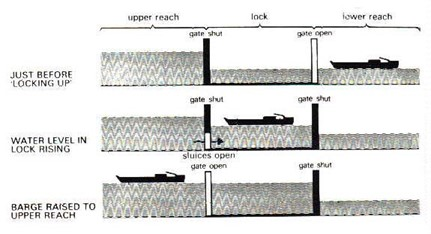
\includegraphics[scale=0.65]{sluismodel.jpg}


Uit deze afbeelding blijkt het volgende:
Hoogteverschip t.o.v NAP
2 sluisdeuren
stoplichten
Uit een onderzoek naar de werking van de verschillende sluizen in nederland wordt rekening gehouden met de aanmelding van sluizen en de gebruiktstijd van sluizen.

Met de aanmelding van schepen wordt omschreven welke acties er door de schipper de sluismeeter moet worden gedaan om de positie, tijdstip en lengte van een invarendship te communiveren.

Met de gebruikstijd wordt  de daadwerkelijke tijd aangeduid waarin het scheepsverkeer/waterverkeer gebruik kan maken van de sluis en onder welke voorwaarden zoals wachttijd, gewicht, terugvaarmogelijkheden etc).

\subsection{Requirements}
Directe requirements van opdrachtgever:\\
Na grondige analyse van het Nederlandse sluizenpark is gebleken dat renova-tie van een groot aantal sluizen noodzakelijk is.  Een eerste verkenning heeft onsgeleerd dat het gecombineerd renoveren en automatiseren van het Nederlandsesluizenpark een aanzienlijke verbetering kan opleveren t.a.v.:\\
- veiligheid\\
- efficientie\\
- capaciteit\\
- onderhoudskosten\\
- duurzaamheid\\
In het kader van het onlangs afgesloten klimaatakkoord heeft de Nederlandseoverheid  daarom  besloten  over te gaan tot een ingrijpende renovatie van dediverse sluizen die ons land rijk is. Op het ministerie van infrastructuur en waterstaat is helaas onvoldoende kennis van ict en systemen aanwezig om eenen ander uit te voeren. Wij vragen u een model (of een onderling samenhangend aantal modellen)aan  te leveren, opdat ontwerpen van verschillende, volledig geautomatiseerde sluizen in de toekomst gerealiseerd kunnen worden.\\\\
Eigen inbreng van deze requirements:\\
Wij gaan er van uit dat het volgende van ons verwacht wordt:\\
Maak een model dat als template dient gebruikt te worden voor het automatiseren van verschillende soorten sluizen. Verder moeten overwegingen gemaakt worden die goed onderbouwd zijn.\\\\ Aangezien er van ons alleen een model verwacht wordt, zullen wij ons geheel focussen op de fundamentele werking van de sluis en hierbij zullen wij ons dus niet bezig  houden met fysieke eisen zoals veiligheidshekjes en borden. Onze focus ligt geheel op de werking van de sluis; elke state waar de sluis zich in mag bevinden en welke beslissingen de sluis moet maken op basis van bestaande protocols en benoemde eisen. \\\\
Deze requirements zullen hieronder uitgewerkt worden, per sluisonderdeel, deze bestaande uit de sluisdeuren, de sloplichten, de waterpomp en de boten.\\




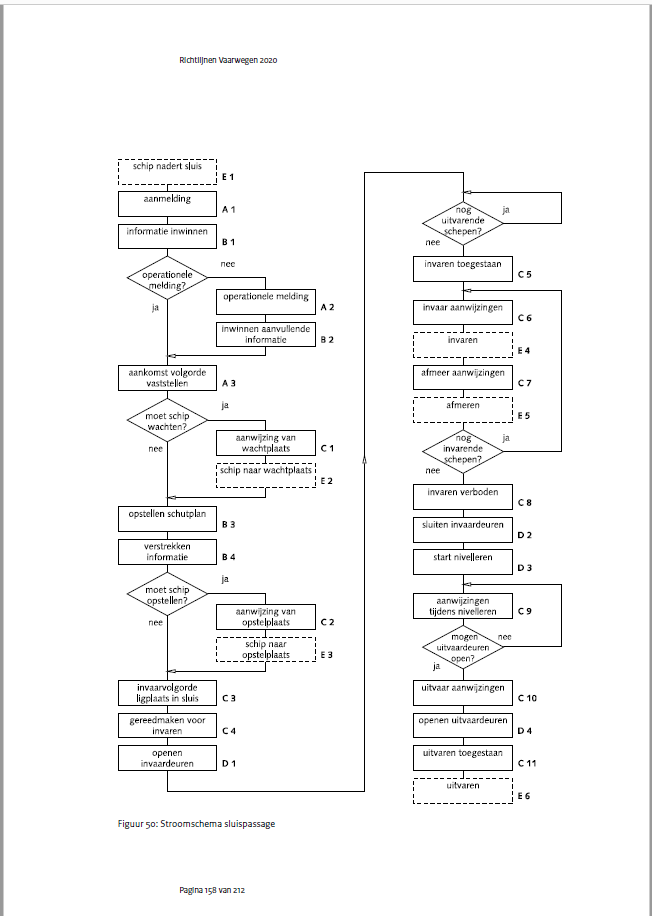
\includegraphics[scale=0.65]{sluispassage.png}


\begin{itemize}
	\begin{minipage}{0.4\linewidth}
		\item Vooraanmelding
		\item informatie inwinnen
		\item operationele melding
		\item aankomst volgorde
		\item aanwijzen wachtplaats
		\item verstrekken informatie
		\item aanwijzen opstelplaats
		\item opstellen schutproces
		\item verstrekken informatie
		\item invaarvolgorde en ligplaats in sluis
		
	\end{minipage}
	\begin{minipage}{0.4\linewidth}
		
		\item gereedmaken voor invaren
		\item openen invaardeuren
		\item invaren toegestaan
		\item aanwijzingen voor invaren
		\item aanwijzingen tijdens afmeren
		\item invaren verboden
		\item sluiten invaardeuren
		\item start nivelleren
		\item stop nivelleren
		\item aanzwijzingen voor uitvaren
		\item openen uitvaardewuren
		\item uitvaren toegestaan
		
	\end{minipage}
	\begin{minipage}{0.4\linewidth}
		\item uitvaren
		\item operationele afmmelding
		\item utvaren verboden
		\item aanwijzing invaren nieuwe schepen
		\invaren verboden
		\deuren gesloten
	\end{minipage}
\end{itemize}


\subsection{Notities die verwerkt moeten worden}

moet de intitial state altijd in een loop zitten in uppaal?
wat zijn urgent channels?
rampen? er staat wel iets in de planning maar kan geen lessen of verdere documentatie of requirements terug vinden?	


gesprek wessel:
main controller slim dat direction een bool is. 
pomp is te slim, zoiu alleen maar aan of uit moeten gaan, of nog weg en in pompen maar meer niet. niets met waterlevel en aantal schepen.
schip: niet doen. als een schip zich aanmeld, dan gebeuren er dingen, maar gaat hij naar binnen? je weet niet wat dat schip gaat doen want menselijk gedrag. beter niet het schip uitgebreid maken, maar eerder de sluis. te veel aannames.

wessel model: alleen als wachtrij vol zit, doet de sluis iets.
deur heeft een parameter zodat er meerdere deuren in de simulator neergezet kunnnen worden. ook bij wachtrij.

stoplichen kunnen er wel in maar als je simpeler wilt, gaan die als eerste weg.
zes variabelen model is voorgesteld maar niet goed op gereageerd. alleen er van af weten is genoeg.
rampen alleen voor persoonlijk verslag





 
\{Liveness}
Liveness properties are of the formn: something will eventually happen, e.g. when pressing the on button of the remote control of the television, then eventually the television should turn on. Or in a model of a  communication protocol, any message that has been sent should eventually be received.
\paragraph{Fairness}
\paragraph{Security}
Safety propertires are of the form: "something bad will never happen". For instance, in a model of a nuclear power plant, a safety propertymight be, that the operating temperature is always (invariantly) under a certain threshold, or that a meltdown never occurs. A variation of this property is that "something will possibly never happen".
For instance when playing a game, a safe state is one in which we can still win he game, hence we will possible not loose.
The system cannot reach states or enable events that are fornidden by the requirements
\paragraph{Performance}
There requirements limit the maximum time to perform when no recoverable errors occur.



\paragraph{brainstorm 22-5-2022}

\subparagraph{invaardeuren en uitvaardeuren}
Gaan we uit van binnendeuren en buitendeuren? Er ontstaat dan een extra ruimte in de sluis. Hoeveel schepen kunnen in deze ruimte? Wat is de maximale wachtreij in deze ruimte en wat zijn de verkeersregels in deze nruimte?
\subparagraph{invaarstoplicht en uitvaarstoplicht}
Als invaren is toegestaan hoe wordt dit dan doorgegeven aan de schepen in de sluis? moeten zij dan uit zichzelf wachten of krijgen zij een signaal dat zij wewl/niet mogen uitvaren? En moeten zij dan kiezen voor links, midden of rechts? Of maakt dat allemaal niets uit?

\subparagraph{invaarwachtrij en uitvaarwachtrij}
Als er meerder schepen in een sluiskolk zitten moet het systeem dan rekeneing houden met het schip dat als eerste is ingevaren en/of het langst in de sluis zit?


\subsection{Sluisdeuren en stoplichten}
De sluisdeuren aan weerszijde van de sluis  worden gebruikt om de toegang tot de sluiskolk mogelijk te maken en te bewaken in combinatie met de stoplicht.



\subsection{Waterpomp}
De waterpomp pompt water in de sluis of pompt water weg naar gelang de richting van het ingevaren schip.

\subsection{Boten}
De meeste sluizen die zich in Nederland bevinden zijn schutsluizen; deze sluizen zijn bedoeld om boten, zowel vrachtschepen als pleziervaart afhangend van de locatie van de sluis, te verwerken. Om deze reden gaan wij deze dus ook verwerken in ons model. Mocht een sluis niet bedoeld zijn om boten te verwerken, dan zou dit model alsnog toegepast kunnen worden opp desbetreffende sluis.
Boten worden toegevoed aan de queue. Hoe dit gebeurt, dat ligt aan de specifieke sluis.  Sinds wij een template maken, hoeven wij geen rekening te hounden met hoe de schepen in de queue komen. Het enige wat wij hoeven te doen, is de data verwerken.




\subsection{Specificaties}
Vanuit deze requiremenst kunnen verdere specificaties opgesteld worden.

Even ter duidelijkheid: een requirement beschrijft wat een programma moet doen, en een specificatie beschrijft hoe men van plan is om deze requirements te realiseren.//
Voorbeeld:// Requirement is dat de sluis meerdere boten moet kunnen verwerken; de specificatie zou hier zijn fdat de sluis minstens twee keer zo groot moet zijn dan de grootste boot die door de sluis kan.





\subsection{Requirements voor Het sluismodel}


\subsection{Requirements}
Requirements zijn alleen die eisen die gesteld worden aan het gedrag of de kwaliteit van het systeem om te voorzien in de behoeften van een belanghebbende uit de business.



Initially the clutch is closed
To open the clutch, it takes at least 100 ms and at most 150 ms
To close the cluch, it takes at least 100 ms and at most 150 ms
Initially the gearbox is neutral
To release the gear, it takes at least 100 ms and at most 200 ms.
To set a gear it takes at leasst 100 ms and at mose 300 ms.
The engine is always in a predefined state called initial when no gear is set.
To find zero torque in the engine, it takes at least 1150 ms and at most 400 ms. ut at 400 ms, the engine may enter an error state or find synchronous speed.
The  engine may regulate on synchronous speed in at most 500 ms.
When in an error state, the engine will regulate on synchrobous speed in at least 50 ms.


A gear change should ne performed within 1 seond (P6-p*,P3)
When an error arises, the system will reach a predefined error state marking the error (p9-p11)
The system should be able to use all gears ( p2-p3)
There will be no deadlocked stat in the system(p17)
When the system indicates gear neutral, the engine should  be in initial state (p12)
The gearbox controller will never indicate open or closed clutch when the clutch is closed or open respctively(p14)
The gearbox controller will never indicate gear set or geur neutral wen the gear is nog set or idle respectively (p15)
When the engine is regulating on torque, the clutch is closed (p16)




\subsubsection{Uppaal kripke structuren}
















\subsubsection{Functionele en niet-functionele eisen}

\subsubsection{specificaties}

\subsubsection{Het vier variabelen model}
Systemen (met daarin software) en de bijbehorende vier variabelen:
\subsubsection{Monitored variabelen}
: door sensoren gekwanticeerdefenomenen uit de omgeving
\subsubsection{Controlled variabelen}
door actuatoren bestuurde fenomenen uit de omgeving
\subsubsection{Input variabelen}
\subsubsection{Output variabelen}




\subsubsection{Aankomst, uitvoering, vrijgave}


\subsubsection{ontwerp}


\subsubsection{Onderdelen}
Op basis van de schets kunnen we vaststellen dat een sluismodel uit de volgende onderdelen bestaat.

\begin{enumerate}
\item Een tweetal sluisdeuren. 
\item Een sluiskolk waarin de schepen in- enuitvaren
\item een stoplicht om een signaal af te geven voor invaren en uitvaren.
\item Een nivelleermachine zorgt ervoor dat het water in de sluis op het gewenste niveau wordt gebracht
\item Een control-system dat ervoor zorgt dat de opdrachten van de sluisbeheerder (geautomatiseerd) worden uitgevoerd
\end{enumerate}
\subsubsection{Werking}

Een schip komt aanvaren en meld zich aan bij de sluismeester. De sluismeester geeft een signaal aan het controlsystem voor het openen van de sluisdeuren, nadat geccontroleerd is of de nivelleermachine al klaar is. Als er ruimte is voor een invarend schip mag het schip dat zoich heeft aangemeld en toestemming heeft  in de sluis varen. Op het moment dat de sluis vol is gaan de sluisdeuren dicht. Eenmaal afgesloten kan de nivelleermachine beginnen om het water in de sluiskolk op het gewenste waterpeil te brengen. Als dit nivelleerprces is afgerond geeft  het controlsystem daan da de sleusdeuren open kunnen.  Als de sleusdeuren open zijn en het uitvaarsignaal is op groen dan moet het schip in de sluis de sluis uitvaren.
\paragraph{extra cases}
Uit het zojuist genoemnde scenario valt het volgende op te maken.
\begin{enumerate}
\item Een schip geeft een signaal aan een sluismeester.
\item Er wordt gekeken of er wel plek is in de sluis .
\item Er wordt gekeken of de nivelleermachine is afgerond.
\item Er wordt gekeken wat het niveo van de waterpeil in de sluiskolk is.
\item Er wordt gekeken of de sluisdeuren gereed zijn voor invarende schepen.
\end{enumerate}
\paragraph{Aandachtspunten}
\begin{enumerate}
\item Voorrang tussen schepen onderling in de sluis?
\item Hoe lang mag een schip zich in de sluis bevinden?
\end{enumerate} 




\subsection{Afbakening}
\begin{itemize}
\item Wat doet de sluis niet.
\item De sluiss houdt geen rekening met links of rechtsrijdend verkeer vanuit de zeevaart
\item De sluis heeft geen queue met daarin een id gekoppeld aan de sluis.
\item De waterpomp wordt alleen aan en uitgezet
\item De waterpomp houdt geen rekening met waterstand
\item Houdt geen rekening met een schip in de sluis dat is blijven hangen.

\end{itemize}






4.2 5 en 6
Het Sluisbeheeerder model wordt getoond in fuguur[]. Het model is een uitbreiding van een schutsluis met alle condities en effecten. De kleuren in de automation verwijizen naar de kleuren in de staat van de automata . De template begint met een initiele lokatie start. De sluisbeheerder initieert het proces door een aangekomen schip te registreren metbehulp van een sychronizate met het channel... over de edge richtng de lokatie "aanmelden." Dit symboliseert een opstartprocedure, ook wordt een functie enqueeu_aanmeldLijst() gebruikt om de juiste waarden te geven aan lokale en globale avariabelen. De lokatie aanmelden regisseert het opstellen van schepen boven of beneden van de sluiskolk. De template Schip synchronizeerd met de template Sluisbeheerder met het channel move_down[id] of move_up[id] en bereikt daarmee de volgende lokatie afhankelijk af de sluis boven of beneden is worden de schepen die in de opstellijst voorkomen, max 2, klaargemaakt voor invaren.. De templates Stoplicht en sluisdeur synchroniseren met de channels ... call_Deur en call_stoplicht.
Het Sluisbeheerder model gebruikt de variabelen clock x, wachttijd_beneden, wachttijd_boven als invariant tussen de lokaties. Om op de hoogete te zijn van de invaar-/uitvaart van de verschillende schepen worden lijsten bijgehouden: list_wachtrij_beneden, list_pos_invaren_beneden, list_schepenInSluis, list_wachtrij_boven en list_pos_invaren_boven.

Het model voltooit de volgende transitie op basis van de waarde van de boolean sluis_bove en sluis_beneden. en de lokale klok variabele x.
Vanaf de locatie invaarverbod_gecontroleerd  wordt gecontroleerd of er nog invarende schepen zijn die in de sluiskolk passen.
Op de lokatie sluiskolk gereed zijn er 1 of meer schepen in de sluis. Als er nog plek is in de sluiskolk n er is nog een schip klaar om in te varen dan wordt dit gecontroleerd, de functie enqueu() voegt het schip toe aan de queue van de sluiskolk. De functie deque() verwijdert de schip van de lijst met invarende schepen. De variabele sluis_boven of sluis_beneden is waar, bij de switch voor het sluiten van deuren en het aanroepe van het stoplicht nr gelang de positie van  de laate binnenvarende schip (boven of beneden). Hierna bereikt de automation sluiskolk_afgesloten.



De lokatie start_nivelleren kiest op basis van de variabelen sluis_boven en de variabelen sluis_beneden het nivellereingsprogramma.
Heet nivellereingsprogramma is Aof B. De keuze voor het programma wordt bepaald door de variabelen van het schip dat in de sluis zit.

De lokatie klaarmaken_voor_openen wordt bereikt als de   hoogte van de sluis  door het nivellereingsprogramma is bereikt.
De positie van de kluis is bepaald door de schepen in de sluis. Vanuit deze lokatie wordt gekeken off de stoplichten gereed moeten worden gemaakt en of de sluisdeuren open mogen.
Hierna volgt een transiie waarin de stoplichte op groen worden gezet en de sluisdeuren worden geopend voor de uitvaart van de schepen in de sluis.
Als alle schepen zijn uitgevaren die uit moeten varen, worden de stoplichten op groen gezet en de deuren gesloten.


De lokatie uitvaren_toegestaan heeft een verbinding(edge) met de lokatie sluis_afsluiten.
Er is een select statement, e:id_t gebruikt als onderdeel van het prototocol om alle uitvarende schepen uit de queue van de sluiskolk te halen, en wordt dan ook gebruikt door de synchronisatie met de channel leave om de schepen uit de sluiskolk te begeleiden. De edge hieraan gekoppeld bevat de functie deque() om de variabelen  van de sluiskolk te resetten.

Vanuit de positie van de sluis worden de schepen gesignaleerd op een invaarverbod en worden de deuren van de sluis gesloten.
De lokatie sluiskolk_afgesloten is bereikt.

Ship [guards, invariants, assignents, synchronizations, properties,aannames]
De template Schip begint bij de Init lokatie. De lokatie is verbonden met de lokatie aangekomen met een edge waarbij een synchronizatie wordt aangeroepen met de template sluisbeheerder. De clock wordt op nul gezet. De lokatie aangekomen is verbonden met de lokatie aangemeld. De edge bevat een synchronizatie waarmee de edge een synchronizatie uitvoert met de template Sluisbheheerder.
De volgende lokatie is  controleren. De edge waarmee de lokatie aangemeld in verbinding staat met de lokatie cnotroleren heeft een synchronisatie voor de template Sluisbeheerder. De lokatie controleren heeft ook een edge met de lokatie wachten. Een schip max maximaal 30 seconden wachten op de lokatie wachten voordat er een mogelijkheid is om opniew in aanmerking te komen voor een controle. Als een schip langer dan 30 tijdseenheden moet wachten de is er een mogelijkheid voor het schip te vertrekken. Hierbij eindigt het schip het invaarproces. Een schip kan dus na aanvaren maximaal 20 seconden wachten om toestemming te krijgen voor een positie invaren anders wordt deze verwezen naar een wachtrij.
Hierna volgdde lokate invarene. De lokatie invarene implieert dat een schip in een invaarproces is dat eindigt in de lokatie gestopt.
Hierop volgd de lokatie nivelleer_start. Hierop wordt een nivelleer_proces gestart. Daarbij is ee synchronisatie met de template Sluisbeheerder.
De lokatie nivelleer_stop is een lokate waarin het nivelleerproces al is gestopt. Van hieruit is er een edge met de lokatie klaar voor vertrek. De edge synchroniseert hiermee met de template Sluisbeheerder.
De lokatie klaar_voor_vertrek is verbonden met de lokatie Init. Met een guard x>=3 tijdseenheden mag een schip vertrekken.


Deur
De deur bevat de volgende lokaties: dicht, openend, open en sluitende.
Een deur sluit niet in een enkele actie. Het proces die een deur dooploopt zijn de processen openend en sluitende. De finale lokaties zijn open en dicht.

Nivelleermachine
De nivelleermachine begint bij de lokatie uit. Met een synchronisatie wordt een nivelleermachine aangezet. De automatie kiest een programma en werkt deze uit in de lokatie bezig. Als ht programma is afgerond volgt de lokatie klaar. Na elk nivelleerproces wordt de machine uitgezet

Stoplicht
Een stoplicht heeft twee lokaties: rood en groen.


\subsection{Template}



\subsection{Verificatie}
     De safety en reachability requirements die formeel zijn gespecificeerd worden in Uppaal geverifieerd met de A en E state formule. Andrerere opreratoren zijn



CTL formulas are based on the following operators:
A (\on every path")
E (\there exists a path")
X (\next time")
G (\globally" or \always")
F (\eventually" or \nally")
U (\until")
R (\release")



Deze zijn als volgt:
\newline
\newline
A[] not maincontroller.rd1 imply
\newline
\newline
A[] maincontroller.rd1 imply
\newline
\newline
A[] not deadlock imply
\newline
\newline
E<> maincontroller.rd1 imply
\newline
\newline
E<> maincontroller.s7
\newline
\newline
E<> maincontroller.s7d
\newline
\newline

\subsection{Formele specificaties}

\paragraph{Safety}
Safety Properties are used to verify that something
bad will never happen. Dit kan worden gespecificeerd met de volgende vergelijking

\aqcap\\

\square ( a_0 \implies (( \lnot a_2 \wedge \lnot a_3 ) \mathcal{U} a_1 ) \vee ( \lnot a_2 \wedge \lnot a_3 )) \\

AG(p)
M, s \models AG(p) $\Leftrightarrow$     \forall \pi \in  \sqcap (M,s) \cdot \forall i \cdot M,\pi[i] \models p\\

EG(p)
M, s \models EG(p) $\Leftrightarrow$     \exists \pi \in  \sqcap (M,s) \cdot \forall i \cdot M,\pi[i] \models p\\

AF(p)

EF(p)

AX(p)

EX(p)

A(p \cup q)
M, s \models  A(p \cup q)   $\Leftrightarrow$     \forall \pi \in  \sqcap (M,s) \cdot \exists k \cdot M,\pi[k] \models q \wedge ( \forall i \leq k \cdot M,\pi [i] \models p)\\
E(p \cup q)

A(p \Re q)

E(p \Re q)

\forall x \, (P(x) \to Q(x)) & premise \\
\forall x \, P(x) & premise \\\hspace*{-30pt} \\


P(x_0) & $\forall x \, \mathrm{e}$ 2 \\
Q(x_0) & $\to \mathrm{e}$ 3, 4 \\

\forall x \, Q(x) & $\forall x \, \mathrm{i}$ 3--5 \\







\{a,b\} or \set†{a,b} \\
\langle a,b \rangle or \gens†{a,b} \\


f \colon A \to B \\

f \circ g \\
x \mapsto f(x) \\

\begin{align*}
	f \colon \mathbb{R} &\to \mathbb{R} \\
	x &\mapsto x^2
\end{align*}


\newline \\
M, s \models p $\Leftrightarrow$ p \in L(s) \\
M, s \models \not f1 $\Leftrightarrow$ M, s \nvdash f1 \\
M, s \models f1 \vee f2 $\Leftrightarrow$ M,s \models f1 or M,s \nvdash f2 \\
M, s \models f1 \wedge f2 $\Leftrightarrow$  M,s \models f1 and M,s \nvdash f2 \\
M, s \models \mathrm{E} g_{1} $\Leftrightarrow$ there is a path \pi  from ~  s ~   such ~  that  ~ M, \pi \models g1 \\
M, s \models p $\Leftrightarrow$ for every path \pi  ~ starting from  ~  s, M, \pi \models g1 \\
M, s \models p $\Leftrightarrow$ s is the first state of \piand M, s \models f1 \\
M, s \models \not g_{1} $\Leftrightarrow$ M, \pi  \nvdash g1\\
M, s \models p $\Leftrightarrow$  M, \pi  \models g1  or  M, \pi  M, \pi  \models g2\\
M, s \models p $\Leftrightarrow$ M, \pi  \models g1  and  M, \pi  M, \pi  \models g2 \\
M, s \models p $\Leftrightarrow$ M, $\pi^{1}$ \models g1 \\
M, s \models p $\Leftrightarrow$ there exists a k \ge 0, such that  ~ M, $\pi^{k}$  \models g1\\
M, s \models p $\Leftrightarrow$ for all i \ge 0,M,$\pi^{i}$ \models g1 \\
M, s \models g1 \bugcup g2 $\Leftrightarrow$ ~  there  ~ exists  ~ ak  ~ \ge  ~ 0 ~  such ~  that  ~ M,  ~ $\pi^{k}$ \models g2\\
and  ~ for  ~ all ~  0  ~ \le j < k, M,$\pi^{j}$ \models g1
M, s \models p $\Leftrightarrow$ for all j \ge 0, if for ~  every  ~ i < j,M,$\pi^{i}$ \nvdash g1 then M,$\pi^{j}$ \models g2\\


\paragraph{Reachability}
Reachability properties are used to check whether
a given state formula can be satisfied by some
reachable state.

\paragraph{Liveliness}
Liveness properties are used to verify that
something eventually will hold
\paragraph{Security}

\paragraph{Performance}

%%%%%%%%%%%%%%%%%%%%%%%%%%%%%%%%%%%%%%%%%%%%%%%%%%%%%%%%%%%%%%%%%
 We think of thevariables innV as the present sate variables and the variables in V'as next state variables. Each variable v i V has a corresponding next state variable in V', which we denote y v'. A valuation for the variables in V and V' can be vieuwed as designating an ordered pair of states or a transition, and we can represent setsof these valuations using formulas as above. We refer to a set of pairs of states as a transition relation. If R is a transition relation, then we write R(V,V') to denote a formula that represents it.
 In order to write specifications that describe properties of concurrent systems we need to define a set of atomic propositions AP. Atomic propositionswill typically have the form v=d where v \in V and d \in D. A proposition v =d will be truein a state s if s(v)=d. Whenv is a variable over the  boolean domain{True,False}, it is not necessarly to include both v = True and  v = False in AP.We will write v to indicate that s(v)=True and \neq v to indicate that s(v)=False.
 We now show how to derive
 
 blz 16
 
 We now show how to derive Kripke M=(S,S_0,R,L) from the first order formulas S_0 and R that represent the concurrent system.
 The set of states is hthe set of all variations	for V
 the set of initial states S_0 is the set of all valuations s_0 for V that satisfy the formula S_0
 let s and s' be the two states, then R(s,s') holds if R evaluates to True when each v \in V is assigned the value s(v) and each v' \in  V' is assigned the value s'(v).
 The labeling function L: S \to  $\2^{AP}$ is defined so that L(s) is the subsetof all atomic propositions true in s. If v is a variable over the boolean domain, then v \in L(s) indicates that s(v)=True, and v $\notin$  L(s) indicates that s(v)=False.
 L: S \to  $\2^{AP}$  is a function that labels each state with the set of atomic propositions true in that state\\
 
Because we require that the transition relation of a kripke structuer us always total, we must extend the relation R if some state s has no successor. In this case, we modify R so that R(s,s) holds.
To illustrate the notions defined in this section we consider a simple system with variables x and y that range over D={0,1}. Thus, a valuation for the variables x and y is justa pair (d_1, d_2) \in D x Dwhre d_1 is the value for x and d_2 is the value for y.

blz 33
Fairness
A fairness constraint an be an arbitraty set of states, usually described by the formula of the logic. if fairness constraints are interpreted as sets of states, then a fair path must contain an element of each fairness constraint infinetely often. If fairness constrants are interpreted	 as CTL formula, then a path is fair if each constraint is true infnetely often along the path. The path quantifiers in the logic are then restricted fair paths.
Formally, a fairkripke structure is a 4-tuple M = (S,R,L,F), where S, L and R are  defined as before and F \subseteq  $\2^{S}$  is a set of fairness constraints ( often called Buchi acceptance conditions) Let \pi = s_0,s_1 be a path in M. Define 
inf(\pi) = {s| s=s_i for infinitely many i}.

We say that \pi is fair if and only if for every P \in F, inf(\p) \cap P \neq $\emptyset$. The semantics of CTL* wth respect to a fair kripke structure is very similar to the semantics of CTL* with respect to ordinary kripke structure. We will write M,s \models_F f to indicate that the state formula f is true in state s of the fair Kripke structure M. Similarly, we write M, $\pi$ \models _f g to indicate that the path formula g is true along path \pi  in M. Only clauses 1, 5 and 6 in the origial semanticss change.
1. M, s \models  _f p  $\Leftrightarrow$ there exists a fair path from s and p \in L(s)
5. M, s \models  _f p  $\Leftrightarrow$ there exists a fair path \pi starting from s such that \pi \models _f g1
6. M, s \models  _f p  $\Leftrightarrow$ for all fair paths \pi starting from s, \pi \models _f g1

To illustrate the use of fairness, conider again the communication protocol for reliable channels. There is one fairness constraint for each channelthat expresses the reliability of that channel. A possible choice for the fairness constraint associated with channel i is the set of states that satisfy the formula \neq send \vee  receive_i. Thus, a computation path is fair if and only if for every channel, infinitly often either a message is received. Other notions of fairness are dealt with in[116].
blz 36
ctl model checking

The model checkingproblem is easy to describe. given a kripke structure M =(S,R,L) that represents a finite-state concurrent system and a termporal logic formula f expressing some desired specification, find the set of all states n S that satisfy f: {s \in S | M, s \models f} \\
Let M = (S,R, L) be a kripke structur. Assume that we want to determine which states in S satisfy the CTL formula f. The algorithm will operate by labeling each state s with the set label(s) of subformulas of f which are true in s. Initially, label(s) is just L(s). The algorithm then goes through a series of stages.During the ith stage, subformulas with i-1 nested CTL operators are processed. When a subformula is processed, it is added to the labelig of each state in which it is true. Onze the algorithm terminates, we will have that M, s \models f iff f \in label(s)
blz 40
Fairness constraints
In this subsection we show how to extendthe CTL model checking algorithmto handle fairness constraints. Let M = (S,R,L,F) be a fair kripke structure. Let F = {P1, ..., P_k} be the setof fairness constraints. We will say that a strongly connnected component C of the graph of M is fair wth respect to F if and only if for each P_i \in F, there is a state t_i \in (C \cap  P_i). We first give an algorithmfor checking EG f_1 with respect to a fair structure. In order to establish the correctness of this algorith, we need a lemma that is analogous to Lemma 1.As before, let M' be obtained from M by deleting from S all of those states at which f_1 does not fairly hold. Thus, M'=(S',R',L',F') where $\S^{'}$ = {s \in S | M,s \models F f1}, R' = R|_S'xS', L' = L|_s;, and F' ={ P_i \cap S' | P_i \in F}.

Lemma 2 M,s \models F EG f1 iff the followingtow conditions are satisfied:
1. s \in S'
2. There exists a path S' that leads from s to somenode t in a nontrivial fair strongly connected component of thr graph (S',R')

In order to determine if M, s \models f p for some p \in AP, we check M,s \models p \wedge fair using the ordinary model-checking procedure.
blz 68
Fairness in model checking with fixpoint

blz 69

blz 70

blz 71
Counterexamples and whitnesses

blz 72


blz 73


blz 74



blz 121
automata theory
blz 141



blz 171
Equivalence and preorders between systems
blz 172

blz 173


blz 174


blz 175


blz 176


blz 177
simulation relations
blz 178

blz 179

blz 180


blz 232
INvariants
blz 233


blz 234


blz 265

blz 266

blz 267


blz 268 parralel compositioon
Before we consider a reachability problem, we show how real-time systems can be modoeled as parralel compositions of timed automata [3,5]. We assume an interleavingor asynchroneous semantics for this operation. Let A1 = (\sum, S1, $\S^{1}_0$, X_1, I_1, T_1) and A_2 = (\sum_2, S1_2, $\S^{1}_0$, X_2, I_2, T_2) be two timed automata. Assume that the two automata have disjoint sets of clocks, that is X_1 \cap X_2 = $\emptyset$. Then, the parralel composition of A_1, and A_2 is the timed automation:

A_1 || A2 = (\Sigma \cup $\Sigma$_2, S_1 x S2, $\S^{1}_0$ x  $\S^{2}_0$ , X_1 \cup X_2, I, T),
where I(s_1,s_2)=I_1(s_1) \wedge I_2(s_2) and the edge relation T is given by the following rules:

1 For a \in $\Sigma$_1 \cap $\Sigma$_2, if \langle s1,a, \varphi, \lambda_1, s_1' $\rangle$ \in T_1 and \langle s2,a, \varphi, \lambda_2, s_2' $\rangle$ \in T_2 then T will contain the transition \langle (s1,s2), a \varphi , \lambda_1 \cup \lambda_2, (s_1',s_2') $\rangle$
2. For a \in $\Sigma$_1 - $\Sigma$_2, if $\langle$ s, a, $\varphi$, $\lambda$, s' \in T_1 and t \in S_2 then T will contain the transition \langle (s,t),a, $\varphi$, $\lambda$, (s', t) $\rangle$
3. For a \in $\Sigma$_2 - $\Sigma$_1, if $\langle$ s, a, $\varphi$, $\lambda$, s' \in T_2 and t \in S_1 then T will contain the transition \langle (t,s),a, $\varphi$, $\lambda$, (t,s') $\rangle$

Thus the locations of the parralel composition are pairs of locations from the component automata, and the invariant of such a location is the conjunction of the invariants of the component locations. There will be a transition in the parralel compoition for ach pair of transitions from the individual timed automata with the same action The source location of the transition will be the composite location obtained from the source locations of the individual transitions. Te target location will be the compositelocation obtained from the target locations of the individual transitions. The guard will be the conjunction of the guards for the individual transitions, and the set of clocks that are reset will be the union of sets that are reset by the individual transitions. If the action of  a transition is only an action of one of the two processes, then there will be a transition in the parralel composition for each location of the othertimed automation. The source and target locations of the original transition and the location fromthe other automation. All of the other components of the transition will remain the same.

		
blz 269 modelling with timed automata

blz 274 clock regions

blz 280 clock zones

blz 281
Timed automata
A timed automation[8,99] is a finite augmented with a finite set of  real-valued clocks. We assume that transitions are instantaneous. However, time can elapse when the automation is in a state or location. When a transition occurs, some of the clocks ma be reset to zero. At any instant, the reading clock is equal to the time that has elapsed since the lat time the clock was reset. We assume that time passes at the same rate for all clocks. In order to prevent pathological behaviours, we only consider automata that are non-zeno, that is, only a finite number of transitions can happen within a finite amout of time.

A clock constraint, called a guard, is associated with each transition. The transition can be taken only if the current values of the clocks satisfy the clock constraint. A clock cnstraint is also associated with each location of the automation. This constraint i called the invariant of the location. Time can elapse in the location only as long as the invariant of the location is true. An example of a timed automation is shown in Figure 17.1 The automation consists of two locations s0 and s1, two clocks x and y, and "a" transition from s0 to s1, and a "b" transition from s1 to s0. The automation starts in location s0. It can remain in that location as long as the clock y is less than or equal to 5. As soon as the value of y is greater than or equal to 3, the  automation can make an "a" transition to location s1 and reset the clock y to 0. the automation can remain in location s1 as long as y is less than or equal to 10 and x is less than or equal to 8. When y is at least 4 and x is at least 6, it can make a "b" transition back to location s0 and reset x.

The remainder of this section contains a formal semantics for timed automata in terms of infinite state transition graphs[3,8]. We begin with a precise definition of clock constraints. Let X be a set of clock variables, ranging over the nonneative real numbers $\Re^{+}$. Define the set of clock constraints C(X) as follows:
All inequalities of the form x \prec c or c \prec x are in C(X) where \prec is either < or  \leq \sm and c is a nonnegative rational number.
If $\varphi$_1 ad $\varphi_{1}$ are in C(X), then $\varphi_1$ $\wedge$ $\varphi$ is in C(X).

Note that if X contains k clocks; then each clock constraints is a convex subset of k-dimensional Eucledian space.Thus, if two points satisfy a clock constraint, then all of the points	on the line sement connecting these points satisfy the clock constraint.
A timed automation is a 6-tuple A = (\Sigma, S, S_0, X, I, T) such that
\Sigma is a finite alphabet
S is a finite set of locations
S0 \subseteq S is a set of starting locations
X is a set of clocks
I : S \rightarrow C(X) is a mapping from locations to clock constraints called the location invariant.
T $\subseteq$ S x $\Sigma$ x C(X) x $2^{x}$ x S is a set of transitions. The 5-tuple $\langle$ s,a,$\varphi$, $\lambda$, s' $\rangle$ corresponds to a transition from location s to location s' labeled with a, a constraint $\varphi$ that specifies when the transition is enabled, and a set of clocks $\lambda$ $\subseteq$ X that  are reset when the transition is executed.


We will require that time be allowed to progress to infinity, that is, at each location the upper bound imposed on the clocks be either infinity, or smaller than the maximum bound imposed by the invariant and by the transitions outgoing from the location. In other words, it is possible either to stay at a location forever, or the invariant will force the automation to leave the location, and at that point at least one transition will be enabled. For timed automata, these constraints can be imposed syntactically.

A model for a timed automation A is an infinite state transition graph \tau(A) = ($\Sigma$, Q, $Q^{0}$, R). Each state in Q is a pair (s, v) where s \in S is a location and v : X $\rightarrow$  $R^{+}$ is a clock assignement, mapping each clock to a nonnegative real value. The set of initial states Q_0 is given by {(s,v)| s \in S_0 \wedge $\forall$ x  $\in$  X[v(x) =0]}.
In order to define the state transtion relation for \tau(A), we musr first introduce some notation. For $\lambda$ $\subseteq$ X, define v[\lambda := 0] to be the clock assignment that is the same as v for clocks in X - $\lambda$ and maps the clocks in $\lambda$ to 0. For d \in \Re, define v +d as the clock assignment that maps each clock x \in X to v(x) +d. The clock assignment v -d is defined in the same  manner.
From the brief discussion in the introduction, we know that a timed automation has two basic types of transitions:
Delay transitions correspond to the elapsing of time while staying at some location. We write (s, v) $\xrightarrow[]{d}$ (s, v+d), where d \in  $R^{+}$, provided that for every 0 \leq e \leq d, the invariant	l(s) holds for v +e.
Action transitions correspond to the execution of a transition	 from T. We write (s,v) $\xrightarrow[]{a}$ (s', v'), where a \in $\Sigma$, provided that there is a transition $\langle$ s,a, $\varphi$, $\lambda$, s' $\rangle$ such that v satisfies $\varphi$ and v=[$\lambda$:=0].

The transition relation R of \tau(A) is obtained by combining the delay and action transitions. We will write (s,v) R(s', v') or (s, v) $\xRightarrow[]{f(x)}$   (s', v') if there exists s" and v" such that (s,v) $\xrightarrow[]{d}$ (s", v")$\xrightarrow[]{a}$ (s', v') for some d \in \Re.
In this chapter we will describe an algorithm for solving the reachability problem for \tau(A): Given a set of initial states Q_n, we show how to copute the set of all states q \in Q that are reachable from Q_0 by transitions in R. This problem is nontrivial because \tau (A) has an infinite number of states. In order to accomplish this goal, it is necessary to use a finite representation for the infinite state space of $\tau$(A). Developing such representations is the main topic of te following sections.

blz 268 parralel composition

blz 274 clock regions
In the definition	 of timed automata, we allowed the clock constraints that serve as the invariants of locations and the guards of transitions to contain arbitrary rational constants.
We can multiply the constants in each clock constraint by the least common multiple m of the denominators of all the constants to integers. The value of a clock can still be an arbitrary nonnegative real number. Note that applying this transformation can change the clock assignments in the set of reachable states of T(A). Fortunately, this does not cause a mjor problem. Ther reachale states of the original auomation can be obtained from the locations of te transformed automation by applying the inverse transformation, that is, dividing each clock value by m.


Th largest constant in the tranformed in the transformed automation is the product of m and the largest constant in the original automation. Thus, the transformation at worst results in quadratic blowup in the length of the encodings of th lock constraints[3]. This increase in complexity is acceptable, since the transformation simplifies certain operations on clock constraints that will be needed later in the chapter. We will apply this tranformation uniformly to all of th clock constraints that appear in the timed automata the we study. Consequently, in the future we can assume without loss of generality that all constants in clock constraints that we encounter are integers.

In order to obtain a finite representation for the infinite state space of a timed automation, we define clock regions[7,8], which represents sets of clock assignments. If two states, which correspond to the  same location of the timed automation A, agree on the integral parts of all clock constraint in the invariant of a location or in the guard of a transition is satisfied or not. The ordering of the fractional parts of the clock values determines which clock will change its integral part first. This is because clock constraints cn involve only integers, and all clocks increase at the same rate.

For example, let A be a timed automation with two clocks x1 and x2. Let s be a location in A with an outgoing transition e to some other location. Consider two states (s,v) and (s,v') in T(A) that correspond to location s. Suppose that v(x1) = 5.3, v(x2)=7.5, v'(x1)=5.5 and v'(x2) = 7.9. Assume that the guard \varphi associated with e is x1 \geq 8 \wedge x2 \geq 10. It is easy to see that if (s,v) eventually satisfies the guard, then so will (s, v').

The value of a clock cn get arbitrarily large; however, if the clock is never compared to a constant greater than c, then the value of the clock will have no effect on the computation of A once it exceeds c. Suppose, for instance, that the block x is never compared to a constant greater than 100 in the invariant associated wit a location or in the guard of a transition.

Then, based on the behaviour of A, it is impossible to distinguish between x having the value 101 and x having the value 1001.
Alur,Courcoubetis, and Dill[7,8] show how to formalize this reasoning. For each clock x \in X, let cx, be the largest constant that x is compared with in the invariant of any location or in the guard of any transition. For t \in  $\Re^{+}$, let ft(t) be the fractional part of t, and let [t] be the integral part of t. Thus, t = [t] + fr(t). We define an equivalence relation \cong on the set of possible clock assignments as follows: Let v and v' be two clock assignments.
Then v  \cong v' if and only if three conditions are  satisfied:

For all x \in X either v(x) \geq cx, and v'(x) \geq gx or [v(x)] =[v'(x)].
For all x,y \in X such that v(x) \leq cx and v(y) \leq cy, fr(v(x)) \leq fr(v(y)) if and only if fr(v'(x)) 
\leq fr(v'(y))
For all x \in X either v(x) \leq cx,
fr(v(x)) =0 if and only if fr(v'(x)) =0.
it is easy to see that \cong does indeed define anequivalence relation. The equivalence classes of \cong are called regions[7,8].  We will write [v] to denote the region which containsthe clock assignment v.Each region can be represented by specifying

1. for every clock x \in X, once clock constraint from the set {x=c | c=0...., cx} $\cup${c -1 < x < c | c=1,.....cx} \cup {x > cx}
2. for every pairof clocks x, y \in X such that c-1 < x< cand d-1<y< d are clock constraints in the first condition, whether fr(x) is less than, equal to, or greater than fr(y).

Figure 17.7 which is taken from [8], shows the clockregions for a timed automationwith two clocks x and y where cx = 2 and cy =1. In this example, there are a total of 28 regions: 6 corner points, 14 open line segments and 8 open regions.

We will use this observation to show that \cong has finite index and, consequently, that the  number of regions is finite. Our proofof this fact is based on the proof given in [8].





Lemma 43
The number of equivalence classes that \cong induces on C(X) is bounded by
|X|! \cdot $2^{|X|}$ \cdot \prod (2xc +2)
proof
An equivalence class [v] of \cong can be described by a tripple	 of arrays i the following manner. For each block x \in X, the array \alpha tells which of the intervals {[],[]}
contains the value v(x). Thus, the array \alpha represents the cloc assignment v if and only if for each clock x \in X, v(x)\in $\alpha$(x). The number of ways to choose \alpha is \prod.


Let X_a be th set of clocks with nonzero fractional part. The array \beta: x_a $\rightarrow$ {1,....|A_a|} is a permutation of X_a, which gives the ordering of the fractional parts of the clocks in Xa with respect to \leq. Thusm the array \bta represents a clock assignment c if and if for each pair x,y \in X_a, if \beta(x) < $\beta$(y) then fr(v(x)) \leq fr(v(y)). For a given \alpha, the number of ways to choose \beta is bounded by |X_\alpha|!  which is bounded by |X|!.

The third component  \gamma is a boolean array indeed by X_a that is used to specify which clocks in X_a have the same fractional part. For each clock c, \gamma(x) tells whether or not the fractional part of v(x) equals  the fractional part of its predecessor in the array \beta. Thus the array \gamma represents a clock assignment v if and only if for each x \n X, \gamma(x) equals 0 exactly when there is a clock \gamma \in X_alpha such that \beta(y) = \beta(x) +1 and fr(v(x)) equals fr(v(y)). The number of ways of choosing \gamma is bounded by the number of boolean arrays over X_\alpha, which is bounded by $2^{|X|}$.
Hence, \alpha encoded the integral parts of he clock assignments, and \beta with \gamma encodes the ordering of their fractioal aprts. It is easy to see that the sets represented bytriples are equivalence of $\cong$ and that every equivalence class is represented by some triple. The bound given in the statement of the lemma is the product of the bounds associated with \alpha, \beta, and \gamma. This completes the proof of the lemma.


The following properties of the equivalence relation $\cong$ are used in later  in this chapter.
Lemma 44
Let v1 and v2 be twoclock assignments1, let \varphi be a clock constraint, and let \lambda $\subseteq$ X be a set of clocks.
1. if v1 $\cong$ v2 and t is a nonnegative integer, then v1 + t $\cong$ v2 +t.
2. if v1 $\cong$ v2, then $\forall$ t1 \in $R^{|+|}$ $\exists$t_2 \in $R^{|+|}$[v1 +t1 $\cong$ v2 + t2]
3. if v1 $\cong$ v2, then v1 satisfies \varphi if and only if v2 satisfies $\varphi$
4. If v1 $\cong$ v2, then v1[$\lambda$:=0] $\cong$ v2 [$\lambda$:=0]

Note that the first property may not hold if t is not an integer. For example, (2.8) $\cong$ (.1, .2),
but (.2, .8) +.3 is not equivalent to (.1,.2) + .3. All of the properties except the second are straightforward to prove and will be left to the reader. A proof if the scond property is sketched below. The proof is not diificultm but it is somewhat tedious. It can be safely skipped when this chapter is read for the first time.



Proof
Assume that v1 \cong v2. We can assume that t1 > 0 because, otherwise, we can simply choose t2=0. Let X{x1,x2,.....,xn}. We can threat v1 as a vector v1 = \langle a1, ......, an $\rangle$, where a_i is the alue of clock x_i in v_1. Similarly, we let v2 = $\langle$ b1, ......, b_n \rangle. Since corresponding clocks have the same integer part, we can assume without loss of generality that 0 \leq a_i < 1 and 0 \leq b_i < 1. Also , assume that the clock values are sorrted into increasing order so that a_1 \leq a_2 \leq ... \leq a_n and b1 \leq b_2 \leq .... \leq b_n.


case 1
Assume that the largest element in v1 + t1 is less than or equal to 1. This case is trivial. We can easilty choose t2 so that v + t1 $\cong$ v2 + t2

case 2
Assume that  0 \leq t1 < 1. Let the first element of v1 +t1. That is greater than or equal to 1 be a_k+t1. Chhoose \in so that \in =0 if a_k+t_1 =1 and so that 0< \ni < b_k-b_k-1 if a_k+t_1 > 1. Note that b_k_-1 < b_k = b_k-1, then a_k=a_k-1 and a_+t_1 is not the first elment of v1+t1 that is greater than o equal to 1. We will show that v1+t1 \cong v2+(1+ \in - b_k). In order to show this we will split the vectors into two parts. Let

L1= $\langle$ a_1 + t1, ...., a_k-1 + t1    $\rangle$, and
L2= $\langle$  b_1 + (1 + \in - b_k), ..., b_k-1 + (1+ \in - b_k)  $\rangle$
In each case it is straightforward to show that

1. all of the elements are positive
2. the elements are sorted in increaing order, and
3. all of the elements are less than 1
Because of these conditios it is easy to see that L_1 \cong L_2. Similarly, let 

R_1= $\langle$ a_k + t1, ...., a_n + t1    $\rangle$, and
R_2= $\langle$  b_k + (1 + \in - b_k), ..., b_k-1 + (1+ \in - b_k)  $\rangle$

All of the elements in R_1 and R_2 are greater than or equal to 1. The fractional parts are given by R_1 - 1 and R_2 -1, respectively. For these vectors it is straightforward to show that

1. all of the elements are nonnegative
2. the elements are sorted in increasing order, and
3. all of the elements are less than 1

Moreover, an element in one vector is 0 if and only if the corresponding element in the order vector is 0. Thus R_1 -1 \cong R_2 -1. It follows immediately that R_1 $\cong$ R_2.
It is not difficult to see that the fractioal parts of R_2 precede the fractional parts of L_2.
Let i  \geq k and j < k. Then
b_i +  (1 + \in - b_k) -1 \leq b_j + (1+ \in - b_k).
is equivlent to b_i - b_j \leq 1, which is obviously true. The same relationship holds for the fractioal parts of R_1 and L_1, that is.
a_i + t_1 -1 \leq a_j + t_1.

hence , we obtain R_1 $\cdot$ L_1 \cong R_2 \cdot L_2, where "\cdot" is concatenation of vectors. This shows that for all t_1 with 0 \leq t1 < 1, there exits a t2 such that v_1 + t_1 \cong v2 + t_2 and completes the proof of 



case 3
Finally, supppose that t_1 \geq 1. Let t1'= t_1 - [t_1], so that 0 \leq t_1 < 1. Find t_2 such that v_1 + t_1 \cong v2 + t2. Then:
v1 + t1 + [t1]  \cong v2 + t2 + [t1].

If we choose t2 = [t1], then we have v1 + t1 \cong v2 + t2 as required. This completes the proof of the second property.

The equivalence relation \cong over clock assignments an be extended to an equvalence relation over the state space of T(A) by requiring that equivalent states have identical locations and equivalent clock assignments: (s,v) \cong (s', v') if and only if s = s' and v \cong v'. The key property of he equivalence reltion \cong is given by the following lemma [5]:


Lemma 45
If v1 \cong v2 and (s, v_1)  $\xrightarrow[]{a}$ (s', v'). The transition \langle s, a, \varphi, \lambda, s' \rangle  that takes state (s, v1) to state (s', v1') corresponds to two transiions of the timed automation.

Proof
Assume that v1 \cong v2 and (s, v1)  $\xrightarrow[]{a}$ (s', v'1). The transition \langle s, a, \varphi, $\lambda$, s' $\rangle$ that takes state (s, v1) to state (s', v'1) corresponds to two transitions of the timed automation:

a delay transition (s, v1)  $\xrightarrow[]{d1}$ (s, v_1 + d_1) for some d_1 \geq 0, and
an action transition   (s, v1 +d1)  $\xrightarrow[]{a}$ (s', v_1') such that v_1 + d_1 satisfies \varphi and v'_1 = (v_1 + d_1)[\lambda :=0].



Since v1 \cong v2 and v1 satisfies I(s), v2 also satisfies I(s). Furthermore, there exists d2 \geq 0 such that v1 + d1 \cong v2 + d2. Since v1 + d1 satisfies I(s), v2 +d2 also satisfies I(s). Because the clock constraint I(s) is convex and is satisfied by both v2 and v2 + d2, I(s) must be satisfied by v2 + e for all e such that 0 \leq e $\leq$ d2. Consequently, the delay transition (s, v2)  $\xrightarrow[]{d2}$ (s, v2 +d2) is legal.

Since v1 + d1 \cong v2 +d2, both v1+ d1 and v2+ d2 must satisfy the clock constraint for the guard $\varphi$. Thus, the transition $\langle$ s, a, $\varphi$, \lambda , s' \rangle myst also be enabled in the state  *s, v_2 + d_2
. Let v'_2 = (v_2 +d_2)[\lambda :=0]. Then v'_2 is equivalent to v'_1. Hence, there is an action transition (s, v_2 + d_2)  $\xrightarrow[]{a}$  (s', v'_2). Combining the delay transition with the action transition, we get (s, v_2)  $\xrightarrow[]{a}$ (s', v'_2) as required.

As a result of the lemme, we can conostruct a finite state transition raph that is  bisimilaion equivalnt to the infinite state transition graph T(A). The finite state transition graph is called the region graph of A[7,8] and is denoted by R(A). A region is a pair (s, [v]). Since \cong  has a finite index, there are only a finite nuber of regions. The states of the region graph are  the regions of A. The construction of R(A) will have the property that whenever (s,v) is a state of T(A), the region (s, [v]) where s_0 is an initial state of A and v_0 is a clock assignment that assigns 0 to every clock. The transition relation of R(A) is defined so that bisimulation equivalence is guaranteed. There will be a transition labeled with a from the region (s,[v]) to the region (s', [v']) if and only there are assignments $\omega$ \in [v] and $\omega$' \in [v'] such that (s, $\omega$) can make a transition to (s', $\omega$')

We summarize the construction of the region graph R(A) below. Let A = ($\sigma$, S, S_0, X, I, T) be a timed automation. Then,
The states of R(A) have the form (s, [v]) where s \in S and [v] i a clock region
The initial states have the form (s_0, [v]) where s_0 \in s_0 and v(x)=0 for all x \in X.
R(A) has a transition ((s,[v]),a, (s',[v'])) if and only if (s, $\omega$)  $\xrightarrow[]{a}$  (s', $\omega$') for some $\omega$ \in [v] and some $\omega$' \in [v'].
 We can use Lemma 45 to prove bisimulation equivalene.

Theorem 31
We will show that T(A) and R(A) are bisimilar. Define the bisimulation relation B by (s,v)B(s,[v]). It is easy to see that the initial state (s_0, v_0) corresponds o the  state (s_0, [v_0]). Next, we show that for each transtition of T(A), there is a corrresponding transition  of R(A), and vice versa. Suppose first that (s,v)B(s,[v]). Suppose on the other hand that (s,v)B(s,[v]) and that  (s,v)$\xrightarrow[]{a}$(s',[v']). Then there exit $\omega$ \cong v and $\omega$' $\cong$ v' such that (s', v") and (s,v) $\xrightarrow[]{a}$(s', v"). Hence v" $\cong$ $\omega$ $\cong$ v', so [v"] = [v']. By the definition of B, (s', v")
B (s', [v"]), it follows that (s', v")B(s', [v']).




blz 280 clock zones
blz 281 Intersection

blz 281 Clock reset


blz 281 elapsing of time
In principle, the three oeraions on clock zones described above can be used to construct a finite representationof the transition graph T(A) corresponding to a timed automation.


Real-time System = Discrete System + Clock Variables by Rajeev Alur

blz 2 actions
The state of a system changes over time. We refer to the state changes of a
system as actions. An action is a pair (\sigma,\sigma ') of states that consists of a source
state \sigma and a target state \sigma '. Intuitively, if a system is in the source state \sigma,
then the action (\sigma,\sigma ') takes the system into the target state \sigma'. We say that
an action is enabled in its source state and disabled in all other states. Two
actions (\sigma,\sigma '1) and (\sigma,\sigma '2) are consecutive if the second action is enabled in
the target state of the rst action|i.e., if (\sigma '1=\sigma '2). The action (\sigma,\sigma ') is a nul l
action if (\sigma=\sigma ')
.

blz 6 clocks and delays

Formally, the action (\sigma,\sigma ') is a system action if for all clock variables x, either
\sigma '(x) = \sigma(x) or \sigma '(x) = 0; the action (\sigma,\sigma ') is a time action - or delay -if there
is a nonnegative real \delta the duration of the delay|such that \sigma ' = (\sigma,\sigma '). System
actions have duration 0. Every null action is, by denition, both a system action and a delay of duration 0.



blz 7 Clock constraints
Let (\sigma, \delta) be a delay, let \phi be a state predicate, and let \psi  be an action
predicate. The characteristic function of \phi maps each nonnegative real e < \delta to
1 if \phi is true for \sigma + e, and otherwise to 0; the characteristic function of   maps
e to 1 iff \psi   is enabled in \sigma + e. A state or action predicate varies finitely over the
delay (\sigma, \delta) if its characteristic function has nitely many discontinuities in the
interval (0,\delta). Abstractly, we restrict ourselves to state predicates and action
predicates that vary nitely over all delays.


blz 8 Clock-constrained systems
A clock-constrained system S = (\phi, \psi ) is a pair that consists of a timed state
predicate 0|the initial condition of S|and a timed action predicate \psi |the
transition condition of S. The timed behavior \sigma is a behavior of the clock-
constrained system S if (1) the initial condition of S is initially true for \sigma
and (2) the transition condition of S is invariantly true for \sigma. Every clock-
constrained system S denes, then, the set of its divergent behaviors, which is
denoted by [[S]].



blz 9 Clock-constrained programs


blz 10 Delay predicates


blz 11 Real-time systems
A real-time system S = (\phi, \psi, \chi) is a triple that consists of a clock-constrained system (\phi, \psi) and a delay predicate \chi the environment condition
of S. The timed behavior \sigma is a behavior of the real-time system S if (1) \sigma is a
behavior of the clock-constrained system that underlies S and (2) the environ-
ment condition of S is invariantly true for \sigma. Every real-time system S defines,
then, the set of its divergent behaviors, which is denoted by [[S]].

For example, the following real-time system S2 = (\phi, \psi, \chi)
changes the value of m from 0 to 1 at time 3 at the earliest and at time 5 at the
latest:
\phi = (m =0 \wedge x =0)
\psi = (m \geq 3 \wedge m1' =1)
\chi = (m =0 \wedge x < 5 ) \vee (m=1)

blz 12 Real-time executability

blz 13 Real-time programs

blz 15 Sequential real-time processes


blz 17 Concurrent real-time processes


blz 19 Embedded real-time processes

blz 30 Verification of Safety Properties

A safety property is simply a closed set of behaviors.
\begin{equation*}
	\begin{split}
		x &= 1 \\
		y &= 2 \\
		\hline
		x + y &= 3 
	\end{split}
\end{equation*}
%%%%%%%%%%%%%%%%%%%%%%%%%%%%%%%%%%%%%%%%%%%%%%%%%%%%%%%%%%%%%%%%%


 

\hoofdstuk{Conclusie}

Wat hebben alle bovenstaande rampen/ongelukken gemeen? Veiligheid.
Bij de therac waren er diverse problemen: communicatie, doorontwikkeling, controle en toetsing
Was het makkelijk te onderzoeken? Waarom?
Bij de boeing 737 crashes was het probleem van controle en communicatie naar medewerkers
Was het makkelijk te onderzoeken? Waarom?

Uit de evaluatie van de china explosion 2015 tianjin komt naar voren dat communicatie, transparantie en veiligheid niet altijd prioriteit hadden bij de lokale autoriteiten
Was het makkelijk te onderzoeken? Waarom?

Bij de tesla autopilot crashes komen soms onvoldoende onderbouwde ontwerpkeuzes naar voren die niet goed zij  afgewogen tegenover het gedrag van de bestuurder
vlucht 1951
Was het makkelijk te onderzoeken? Waarom?

De ramp in Tsjernobyl toont aan hoe autoriteiten een ramp in de doofpot proberen te stoppen
Was het makkelijk te onderzoeken? Waarom?



Wat heb ik geleerd
Ik heb erg veel geleerd van het veilig opzetten van VPN’s. Een VPN opzettenhad ik namelijk nog nooit gedaan. Het opzetten van SSH en het aanmaken vanVM’s was al bekend. Ook had ik nog nooit met UDP sockets geprogrammeerd.Verder heb ik geleerd hoe ik in de praktijk een VM in een VLAN kan zetten enhoe VLAN’s netwerken van elkaar kunnen scheiden.Het leukste onderdeel van het project, was dat wonderbaarlijk mijn gekozenoplossing elegant werkte. UDP Servers en clients zijn gerealiseerd met minderdan enkele regels logisch scipt. Ik had aan genomen dat het werken met socketsin shell absoluut rampzalig zou uitpakken. Ik ben blij dat het opdracht zo vrijwas, zodat ik experimenteel kon zijn met mijn implementatie.



